\documentclass[pdftex,10pt,b5paper,twoside]{book}
\usepackage[lmargin=25mm,rmargin=25mm,tmargin=27mm,bmargin=30mm]{geometry}

\usepackage[utf8]{inputenc}
\usepackage{graphicx}
\usepackage{float}
\usepackage{bm}
\usepackage{amsmath,amsfonts,amssymb,amsthm}
\usepackage{subcaption}
\usepackage[labelfont=bf]{caption}
\usepackage{listing}
\usepackage[strings]{underscore}

\usepackage{tex/macros}

\setlength\parindent{0pt}
\setlength{\parskip}{\baselineskip}

%%% Local Variables:
%%% mode: latex
%%% TeX-master: "thesis"
%%% End:


\begin{document}

% Assume that the title page is generated automatically, thus jumping straight
% into the abstract.

\chapter*{Abstract}

\textcolor{red}{
  A bunch of abstract.
}

%%% Local Variables:
%%% mode: latex
%%% TeX-master: "../thesis"
%%% End:

\tableofcontents
\listoffigures
\listoftables

\chapter{Introduction}

Reservoir Computing spawned from difficulty of training RNNs. From Reservoir
Computing we now have a lot of physically based reservoirs. Introduce the
sentiment.

Now, with physical reservoirs, we will have to adapt our previous Echo State
Networks to physical morphologies. Does this work?

Spatial networks, can we use existing graph and lattice theory? Can we find
regular structures that exhibit the same characteristics we see in existing
models like ESN/LSM?

\section{Goals}

Research questions:

\begin{itemize}
\item How does the Reservoir Computing paradigm translate to the spatially
constrained topology setting of a physical medium?
\item How do highly regular structures compare in terms of memory capacity,
information processing capacity, and robustness, to that of established models
such as echo state networks?
\item Can we find simple, deterministic weighting schemes for recurrent neural
networks, that are realizable as physical interactions?
\end{itemize}

\section{Overview}

Chapters are about so and so.

%%% Local Variables:
%%% mode: latex
%%% TeX-master: "../thesis"
%%% End:
\chapter{Background}

Related work and the state of the art were reviewed, and identification of
relevant background material was carried out in the project preceding this
thesis \cite{aven_exploring_2019}. This background is herein amended with deeper
insights into the paradigm of physical reservoir computing, and adapted to fit a
thesis rather than an article. Specifically, the main focus is transferred from
physical limitations in general, to the narrower scope of spatial limitations
relating to physical morphology and topology.

\textcolor{red}{
  The chapter covers important material used throughout the text, as well as a
short historical background for context. Talk about sections.
}

\section{Complexity: Order, Chaos and Criticality}

In deeming a physical system able to \textit{compute}, one implies information
storage, retrieval and modification. We are as humans intimately familiar with
the continuous, yet spontaneous computation present in our brains -- our
consciousness. We are less acquainted, however, with the conditions that
\textit{caused} the emergence of such a system.

Spanning a wide range of topics and disciplines, the field of \textit{complexity
theory} seeks answers to this conundrum. An exact definition of ``complexity''
is perhaps ever so elusive, but at its core lies an emergence of behavior
greater than the sum of its parts. Simple, local interactions give rise to
intricate, global patterns. This spontaneous emergence of complex behavior is
ubiquitous in nature. Ranging from convection cells in physics, to swarm and
flock behavior in biology, there is an abundance of interesting phenomena to
study \cite{heylighen_science_1999-1}.

Langton investigated the emergence of computation in cellular automata (CA)
\cite{langton_computation_1990}. His findings indicate a \textit{criticality} as
a condition to support computation. In essence, in between \textit{ordered} and
\textit{chaotic} dynamics, we find a critical phase transition. It is these
systems, intertwining order and chaos, that are of interest.

In systems that are too static, perturbation will fade too quickly. Chaotic
systems, on the other hand, are wildly unpredictable, making them excessively
sensitive. This \textit{edge of chaos} is a recurring theme in the investigation
of the computational capabilities of physical systems. In fact, the edge of
chaos has been found to be of significant in predicting the computational
performance of for neural microcircuit models, consisting of spiking neurons and
dynamic synapses \cite{legenstein_edge_2007}.

Biologically inspired models, most famously the artificial neural network (ANN),
are valuable scientific tools. Oftentimes, finding a suitable set of parameters
for a model will amount to much the same as finding the critical phase
transition between order and chaos. Reservoir computing (RC), a niche framework
within the field of machine learning, is concerned with observing the inherent
dynamics of a ``reservoir'' of local interconnections. Often employing random
neural networks, RC exploits the intrinsic computation emerging from these local
interconnections to solve practical tasks.

\textcolor{red}{
  Should we include any figures? There is much beauty to behold.
}

\section{Reservoir Computing Fundamentals}

Training recurrent neural networks (RNN) is an inherently difficult
task. Gradient descent methods that incorporate loss information become
increasingly inefficient on problems with long-range temporal dependencies. This
inefficiency makes the backpropagation algorithm used with feed-forward
structures less attractive. Specifically, a continuous search in the parameter
space of recurrent networks may cause bifurcations points in the dynamics of the
system, causing non-convergent training \cite{doya_bifurcations_nodate}. To
circumvent this complexity, alternative methods that leave internal weights
untrained have been proposed.

Liquid State Machines (LSMs) \cite{maass_real-time_2002} and Echo State Networks
(ESNs) \cite{jaeger_echo_2001} independently present supervised learning methods
that do not adapt the internal weights of the RNN. Instead, the output is
generated using a simple, memoryless classifier or regressor. This makes the RNN
function much like a kernel in kernel method algorithms, which seeks features
and general relations in datasets to increase separability.

Thus, by projecting into a high-dimensional space, temporal information of an
input may be incorporated in an instantaneous readout. This methodology has been
unified into the research subfield of RC \cite{schrauwen_overview_2007}, in
which the focus is on separating the randomly generated \textit{reservoir} from
the trained readout layer.

Interestingly, there is no need for the reservoir to be an artificial neural
network -- any high-dimensional, driven system exhibiting complex dynamic
behavior can be used \cite{schrauwen_overview_2007}. As long as the dynamics
that governs a given \textit{substrate} can be harnessed through system
perturbation and readout, it can in theory be used as a reservoir.

% (TODO): Correct section reference.
A multitude of substrates have shown promise as reservoirs: dynamical systems
models such as CA \cite{yilmaz_reservoir_2014}, and the more general random
Boolean network (RBN) \cite{snyder_computational_2013}, provide a discrete
alternative to the analogue ESN. Furthermore, a recent surge in physical
reservoir implementations has reinvigorated the field, which is further
introduced in Section \textcolor{red}{ref}.

\section{Echo State Networks}

\subsection{Recurrent Neural Networks}

\textcolor{red}{
  Their use, and why backward edges makes it notoriously difficult to train such
networks.
}

\subsection{Echo State Networks}

\textcolor{red}{
  The inception of reservoir computing as a methodology with Jaeger's Echo State
Network and Maass's Liquid State Machine.
}

\textcolor{red}{
  A section that specifically explains how the default Echo State Networks
function. Some minor details about work that has been done to improve upon the
model, such as intrinsic plasticity, leaking neurons, lateral inhibitions, and
so on. Can/should be adapted from pre-thesis.
}

\textcolor{red}{
  Common tunings, such as input scaling, spectral radius, leakage and
sparsity. Extensions to base model. Bias, output feedback, teacher forced
etc. Also deep ESNs now (most recent, actually quite recent).
}

\textcolor{red}{
  Echo State Property and short-term memory.
}

\subsection{Real World Applications}

The ESN methodology has been applied somewhat successfully to real world
tasks. Approaches include equalizing a wireless communication channel
\cite{jaeger_harnessing_2004}, and short-term traffic \cite{an_short-term_2011},
electric load \cite{song_hourly_2011}, and stock price forecasting
\cite{lin_short-term_2009}. Robot control is also a popular area of research for
RC applications, particularly for motor control and event detection
\cite{aislan_antonelo_learning_2015, harding_evolution_2005,
hutchison_movement_2004}. Perhaps less conventionally, RC has also been applied
in the context of reinforcement learning \cite{bush_modeling_2005}.

However, as the practicality of the paradigm resides primarily in chaotic time
series prediction and classification, this is also its main focus. Furthermore,
recent years have seen an increase in the realization of physical reservoirs to
accompany existing software simulations. An example is a silicon photonics chip
capable of 5-bit header recognition up to 12.5 Gbits$^{-1}$, and is scalable to
even higher bitrates \cite{vandoorne_experimental_2014}. This surge of optimism
has breathed new life into the field of RC, as physical reservoirs pave the way
for new types of integrated chips.

\subsection{Comparison to State of the Art}

Few definitive comparisons between the ESN and similar flavors of the RNN have
been carried out. The long short-term memory (LSTM) \cite{hochreiter_long_1997},
as well as its more recent descendant, the gated recurrent unit (GRU)
\cite{cho_learning_2014}, are mainstays in sequence processing, particularly in
natural language processing. Early experiments demonstrated the ESN methodology
to outperform previous LSTM methods on learning a chaotic attractor by orders of
magnitude \cite{jaeger_echo_2001}, but ESNs have largely remained a secondary
tool outside of chaotic time series prediction and classification.

A recent study compares the promising deep echo state network architecture
(DeepESN) to that of gated RNNs, where an experimental comparison between
recurrent models on multivariate time-series prediction tasks is made
\cite{gallicchio_comparison_2019}. It is established that the DeepESN
methodology outperforms other RNN approaches in their prediction ability on
challenging, real world datasets. The computation time is also lessened about
one order of magnitude compared to fully-trained RNN approaches. Thus, the
adoption of LSTM and GRU in practice may not necessarily be based on performance
suitability, but rather software availability and popularity.

\section{Physical Reservoir Computing}

\textcolor{red}{
  Often used quite interchangeably with ``Evolution in Materio''.
}

\textcolor{red}{
  Anything exhibiting complex dynamic behavior may be used. Explain this, and
why this is, and what implications this carries.
}

\textcolor{red}{
  The emergence of physical substrates as a medium for the reservoir computing
paradigm. Illustrate some of the main topics, like photonics, optoeletronics,
mechanical (coupled oscillators), biologically inspired (ecoli, invitro),
magnetism. Use the survey paper by Tanaka et al.
}

\textcolor{red}{
  It is importance to stress that we are considering alternatives to the
traditional reservoirs in this section. Drive home the point that we are
exploring physical mediums that are wildly different from traditional computers,
where memory and computation and fundamentally separate.
}

\textcolor{blue}{
  ``There are many physical properties and considerations that require
discussion when talking about using any novel material for computation. Here we
focus on four key factors that possess some relevance to substrate-based
reservoirs: (i) a means by which to observe network connectivity and activity,
(ii) assuring non-linearity is present in the system, (iii) methods for
modelling activity and behaviour, and (iv) the impact of environmental
factors.'', in-materio paper, Dale et al.
}

\subsection{Spatial Networks and Topology}

\textcolor{red}{
  Use a previous section on physical reservoir computing to lead into background
on networks that are manifested into a physical space. Talk about previous work,
such as the Minimum Complexity Echo State Network, which has research goals that
very closely resemble that of this thesis.
}

\textcolor{red}{
  Discuss existing theory on spatial networks. Relevant topics may include the
Erdős–Rényi model as a basis for Echo State Networks, then the Waxman model with
its physical restraints, and then a dive further into completely regular
structures such as lattices. Watts-Strogatz.
}

\textcolor{blue}{
  Previous work on topology. For example ``Reservoir Topology in Deep Echo State
Networks'' by Gallicchio et al., ``Optimal modularity and memory capacity of
neural reservoirs'', Rodriguez et al., ``Role of Structure..'', Dale et al.,
``Stability and Topology in Reservoir Computing'', Manevitz et al., and lastly
all of Rodan's thesis on CRJ and deterministically constructed networks.
}

\textcolor{blue}{
  ``Graph Echo State Networks'' and ``Tree Echo State Networks'' by
Gallicchio. \cite{gallicchio_tree_2013}. \cite{gallicchio_graph_2010}. The
possibility of extending neural networks methodologies for learning in domains
of highly structured data representations.
}

\section{Assessing Reservoir Quality}

Designing \textit{good} reservoirs, possessing some set of desired properties,
naturally requires some metric by which we can evaluate and compare. Parameter
sweeps, i.e. our trial and error methods, must be accompanied by sufficient
methods of assessing computational performance.

Evaluation of reservoir quality is split into two different
approaches. Intuitively, measuring the performance of the model on a given
benchmark task is a simple, direct way of assessment. However, to gain an
intuition for a more general, expected performance across multiple benchmarks,
one may measure independent properties of the system, e.g. the spectral radius
of the internal weight matrix. The two approaches are often used in conjunction,
combined to propose an overall quality.

\subsection{Independent Metrics}

\subsubsection{Kernel Quality and Generalization}

Within the RC paradigm we are concerned with producing a complex mapping from
the input stream to some spatial, internal representation, such that a
memory-less, linear readout map may be employed for classification.

The \textit{linear separation property}, or \textit{kernel quality}, measures
ability to separate different inputs \cite{legenstein_edge_2007}. It is an
empirical measure of this complex mapping, denoting the potential diversity of
nonlinear operations carried out by a reservoir. Kernel quality is evaluated by
presenting a reservoir of size $n$ with $m$ different input sequences, and
computing the rank of the resulting $m\times n$ matrix consisting of the
reservoir states resulting at some time step $t$ for the input stream
\cite{busing_connectivity_2010}.

Another metric accompanying the kernel quality is the \textit{generalization
capability} of the reservoir \cite{legenstein_edge_2007}. This metric addresses
ability to generalize already learned functions or filters to new, unseen input,
and is used as an estimation of the VC-dimension of the
reservoir. Generalization capability is evaluated with the same method as kernel
quality, but instead requires input streams that are similar, or belong to the
same class \cite{busing_connectivity_2010}.

A reservoir in the ordered regime will naturally exhibit low values on both
metrics, while both metrics will be high in a network in the chaotic
regime. Thus, in general, reservoirs exhibiting a high kernel quality and a low
generalization rank are desirable, and the difference between the two is
sometimes used as its own metric \cite{busing_connectivity_2010}.

\subsubsection{Short-Term Memory}

Short-term memory capacity was introduced as a quantitative measurement of
linear memory capacity in reservoirs \cite{jaeger_short_2002}. It is a way to
examine the fading memory present in the system, and is measured by attaching
output units to the reservoir, which each are trained to recall some time
delayed version of the input sequence. By measuring how much of the input each
output unit can recover, we can estimate the memory capacity $MC$ by summing
over all time delays. Jaeger defined this as

\begin{equation}
  MC =
  \sum_{k}^{\infty}MC_{k} =
  \frac
  {cov^2(u(t-k), y_k(t))}
  {\sigma^{2}(u(t))\sigma^{2}(y_{k}(t))}
  ,
  \label{stm-eq}
\end{equation}

where $MC$ in general is limited by the reservoir size $N$, such that $MC \leq
N$. High input retention is a desirable property, but an increase in memory
capacity through parameter tuning is often met with a decrease in complex
information processing, due to a universal trade-off between memory and
nonlinearity \cite{dambre_information_2012}.

% (TODO): Not entirely orthogonal from generalization (see Burkow).

% (TODO): Cite "Computational analysis of memory capacity in echo state
% networks" in the methodology section of this specifically for ESNs.

\subsubsection{Memory-Nonlinearity Trade-off}

Experimentation with a wide range of reservoirs has indicated a crucial
interplay between the memory and nonlinearity properties in reservoir operation
\cite{verstraeten_memory_2010}. In fact, the interplay has been uncovered to be
a universal trade-off between depth of memory and nonlinear computation
performed by a dynamical system \cite{dambre_information_2012}.

Thus, analyzing the boundary between an ordered, static regime that provides
memory, and a chaotic, dynamic regime that provides processing, is of vital
importance in the design of reservoirs. Determining the required nonlinearity
for a task is not a simple task, and often benefits from intuition about
nonlinear dynamics. Empirically, it has been shown that the input scaling,
determining the nonlinearity of reservoir responses, and the spectral radius,
scaling the importance of previous states, are the main parameters for
optimization in ESNs, illustrating the significance of the trade-off
\cite{montavon_practical_2012}.

Further formalization of the trade-off has been conducted, accompanied by a
proposition of a mixture reservoir combining both linear and nonlinear
dynamics. Adding a ``pinch of linearity'' is cited to improve performance
considerably \cite{inubushi_reservoir_2017}.

\subsubsection{Further Metrics}

A handful of other methods to assess quality and criticality of reservoirs have
been adapted, including the Lyapunov exponent
\cite{verstraeten_experimental_2007}, the Jacobian of the reservoir
\cite{alippi_quantification_2009}, Fisher information
\cite{livi_determination_2018}, and a separation ratio
\cite{gibbons_unifying_2010}.

In summary, given the vast amount of methods for evaluation, choosing a set of
suitable metrics is a surmountable task. This is especially so, given that few
metrics are entirely orthogonal, and are can be found to strongly correlate in
the prediction of performance \cite{chrol-cannon_correlation_2014}.

\subsection{Benchmarks}

Employing benchmarks to measure the performance of reservoirs is a means to
directly capture performance on specific tasks. Myriads of benchmarks exist
within the field of time series prediction, generation, and classification. The
benchmark spectrum range from simple tasks, to complicated, highly dynamic and
autoregressive time series.

Simpler tasks include the XOR problem of which is not linearly separable
\cite{goos_pattern_2003}, and n-bit temporal density and parity
\cite{bertschinger_real-time_2004}. More complex tasks may range from
recognizing isolated digits in speech \cite{verstraeten_isolated_2005}, to
predicting time series, of which the most popular are the Mackey-Glass time
delay differential equation \cite{mackey_oscillation_1977}, and the nonlinear
autoregressive moving average, NARMA \cite{atiya_new_2000}. Further datasets,
such as the Santa Fe Laser, Hénon Map, IPIX Radar, and Sunspot series datasets
have also been used \cite{rodan_minimum_2011}.

\subsubsection{NARMA - Nonlinear Autoregressive Moving Average}

\begin{figure}[t!]
  \centering
  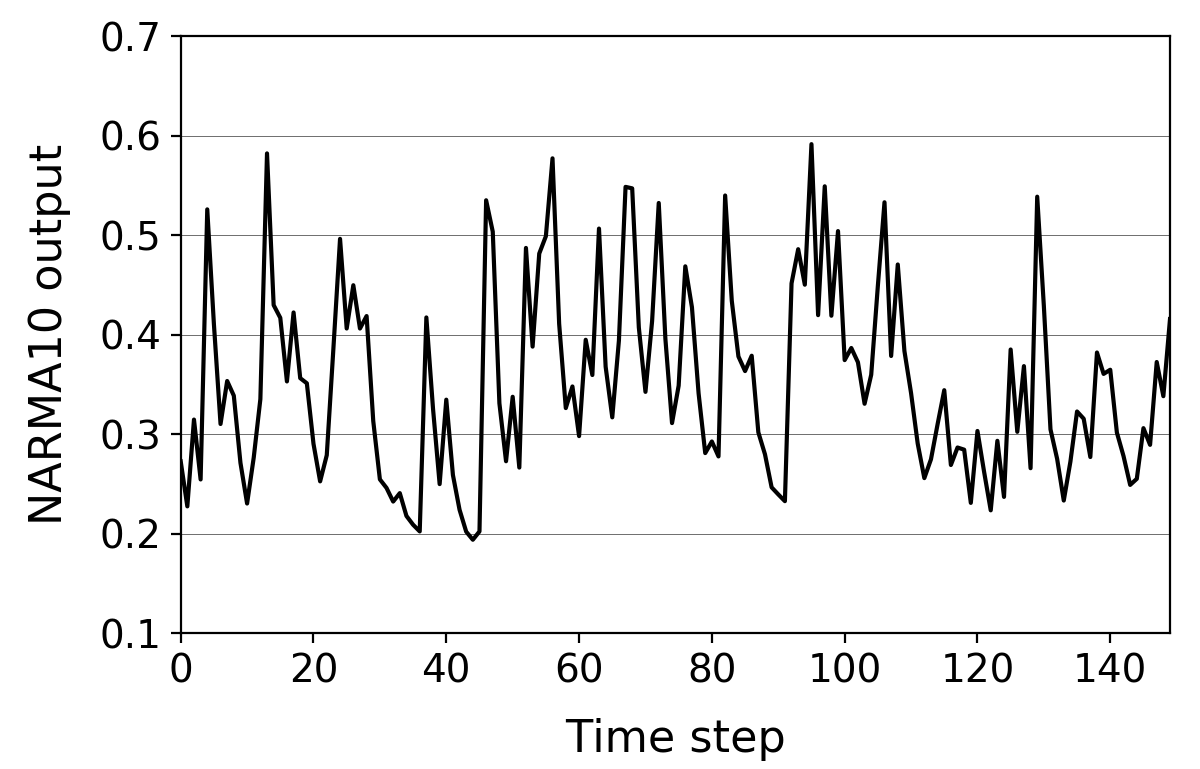
\includegraphics[width=3.0in]{figures/NARMA10.png}
  \caption{
    Example output generated by a 10th-order NARMA system. The autoregressive
moving average nature of the time series is clearly visible.
  }
  \label{fig:narma10}
\end{figure}

The class of time series provided by a nonlinear autoregressive moving average,
most often simply referred to as \textit{NARMA}, is a model commonly used to
benchmark recurrent networks \cite{atiya_new_2000}. Its widespread use yields
baseline performances for well established models, as well as more novel
approaches \cite{verstraeten_experimental_2007, appeltant_information_2011}.

NARMA provides discrete-time temporal tasks, introducing a time-lag of $n$ time
steps, and is given by

\begin{equation}
  y_{t} = \alpha y_{t-1} +
  \beta y_{t-1} \sum_{i=1}^{n}y_{t-i} +
  \gamma u_{t-1}u_{t-n} +
  \delta
  .
  \label{eq:narma}
\end{equation}

Here, $n$ is the order of the system, and common constant parameters are $\alpha
= 0.3$, $\beta = 0.05$, $\gamma = 1.5$ and $\delta = 0.1$. The input $u_{t}$ is
an i.i.d. stream drawn uniformly from the interval [0, 0.5]. The time series is
unstable, and tasks with higher than a 10th-order time lag introduce a
saturation function to produce a bounded sequence:

\begin{equation}
  y_{t} =
  \tanh(
  \alpha y_{t-1} +
  \beta y_{t-1} \sum_{i=1}^{n}y_{t-i} +
  \gamma u_{t-1}u_{t-n} +
  \delta
  )
  .
  \label{eq:narma-tanh}
\end{equation}

\begin{figure}[t!]
  \centering
  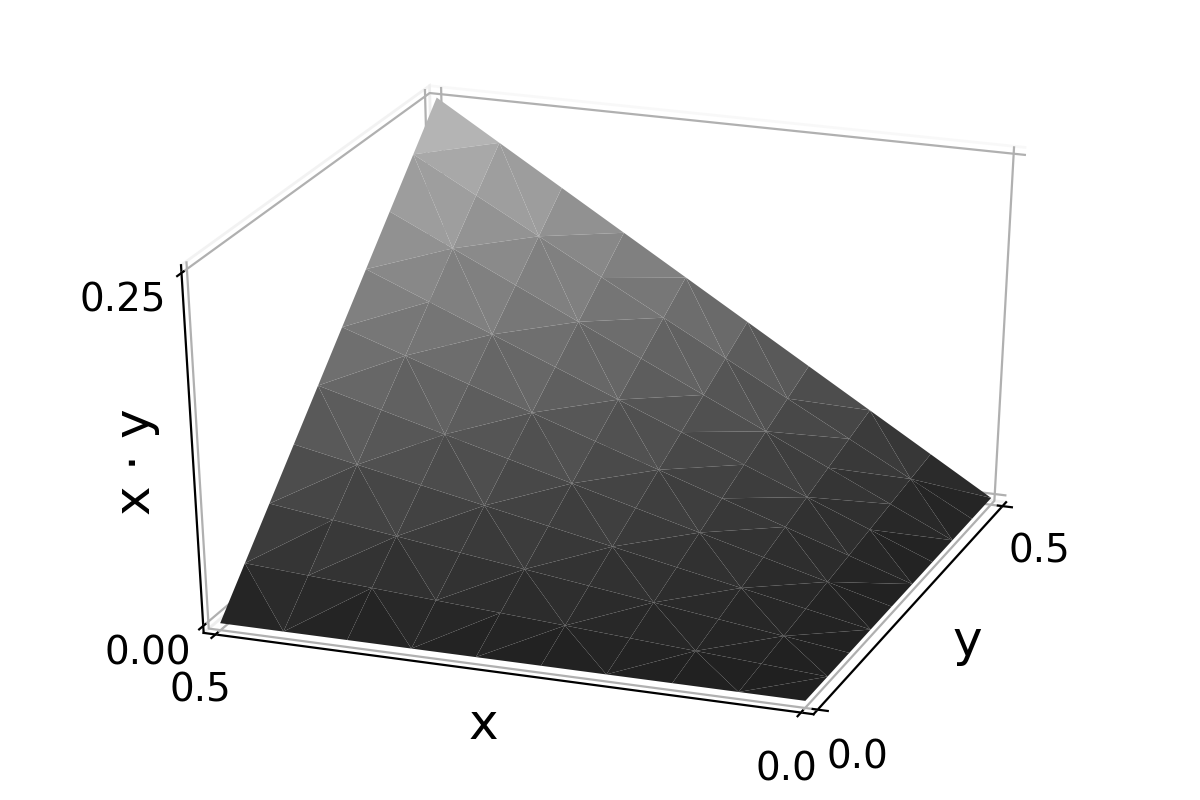
\includegraphics[width=3.0in]{figures/NARMA-nonlinearity.png}
  \caption{
    Nonlinear mapping of the product $u_{t-1}u_{t-n}$ of inputs in the NARMA
time series in Equation \protect\ref{eq:narma}.
  }
  \label{fig:narma-nonlinearity}
\end{figure}

Predicting a NARMA time series, given an input sequence $u$, presents a
challenge of both memory and nonlinearity. This makes NARMA well-suited for
evaluating both the memory capacity and computational power of reservoirs with a
single metric. Reservoirs must necessarily remember input sequences of length
$n$, and should preferably adhere to suitable dynamics on top of this. A
10th-order system is depicted in Figure \ref{fig:narma10}, and a nonlinear
product on the input sequence is shown in Figure \ref{fig:narma-nonlinearity}.

Evaluation of ESN performance on the NARMA10 system is a thoroughly explored
area in the field of RC. Reported NRMSE performances for traditional ESN
reservoirs of size $N = 200$ lie in the range [0.20, 0.25]
\cite{verstraeten_experimental_2007, rodan_minimum_2011,
goudarzi_comparative_2014, jaeger_adaptive_2003}. For some context, using a
shift register containing the input as a reservoir will achieve a minimal NRMSE
of 0.4. To achieve NRMSE values below this threshold it is necessary to
introduce nonlinearity in the reservoir.

%%% Local Variables:
%%% mode: latex
%%% TeX-master: "../thesis"
%%% End:
\chapter{Methodology}

Introduce the baseline Echo State Network that we used, and what types of
training data we used for offline training and so on.

Should we split experiments into multiple sections that all have their own
little mini-IMRAD? Could be helpful to first finish everything related to Waxman
model graphs, finish the discussion, and then lead further on to lattices.

Anyway: for each experiment, describe the experimental setup that was used such
that it may \textit{easily be reproduced}. It has been very helpful when papers
actually provide every relevant parameter such that I could run the experiments
myself.

%%% Local Variables:
%%% mode: latex
%%% TeX-master: "../thesis"
%%% End:
\chapter{Experiments: Random Geometric Graphs}
\label{ch:rgg}

% (TODO): t!
\begin{figure}[t]
  \centering
  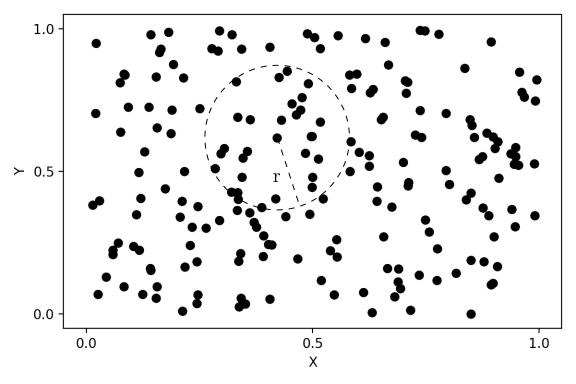
\includegraphics[width=3.5in]{figures/RGG-example.png}
  \caption{
    Example vertices drawn to generate a random geometric graph embedded in a
two-dimensional Euclidean space. The neighborhood radius $r$ of a single node is
shown.
  }
  \label{fig:rgg-example}
\end{figure}

The first idea that springs to mind when considering spatially constrained
graphs, is of course to place the vertices in some metric space. When
investigating spatial reservoirs, it is thus only natural that we begin with the
simplest spatial network model -- the random geometric graph (RGG). Figure
\ref{fig:rgg-example} depicts an example graph.

To construct a reservoir based on the RGG model, we place its $N$ internal nodes
randomly in an underlying metric space $[0, l)^{dim}$, giving each node a
position attribute sampled from a uniform distribution. For any given pair of
nodes $x, y$, we consider the Euclidean distance between them

\begin{equation}
  d(x, y) = \norm{x-y}_{2} = \sqrt{\sum_{i=1}^{dim}{(x_{i}-y_{i})^2}}.
  \label{eq:rgg-dist}
\end{equation}

Nodes are connected only to the nodes within their neighborhood radius $r$,
i.e. where $d < r$. However, since we are interested in the behavior in physical
materials, we set $r = \infty$ to allow full connectivity in all
experiments. Thus, edges are weighted according to several distance functions,
$1/d$, $1/d^2$, and $1/d^3$, to model how the interaction strength diminishes
with distance in many physical substrates. For example, the spins in artificial
spin ice is subject to a magnetic field from all neighboring spins that
diminishes according to $1/d^3$ \cite{jensen_computation_2018}. A dimensionality
of 3, i.e. $[0, l)^{3}$, is used.

\section{Size of the Underlying Volume}
\label{sec:volume-size}

\subsection{Synopsis}

Our first experiment is concerned with the size of the metric space in which we
embed the reservoir, the $l$ of $[0, l)^3$. The behavior of the ESN created will
obviously be affected by the magnitude of the weights of the network edges. A
space that is too small, will result in weights that are too big, and vice
versa.

\subsection{Results and Discussion}

% (TODO): t!
\begin{figure*}[t!]
  \centering
  \begin{subfigure}{.49\textwidth}
    \centering
    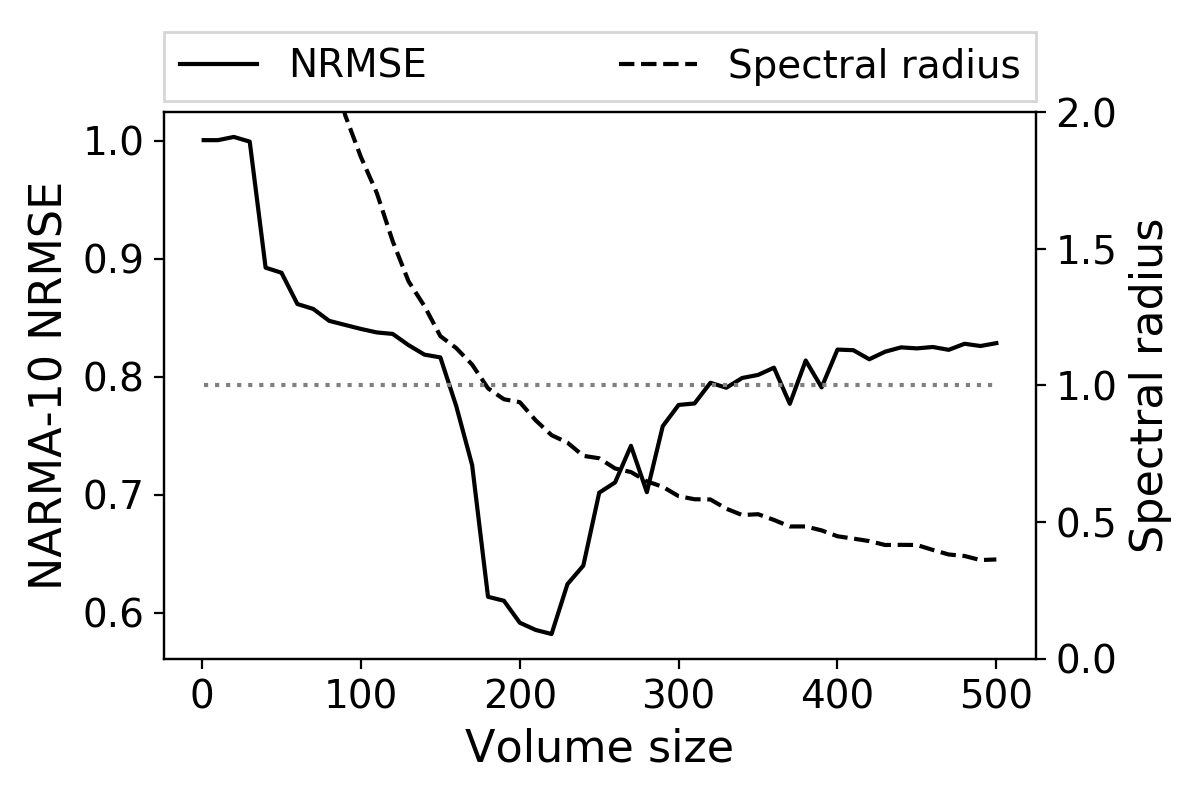
\includegraphics[width=1.0\linewidth]{figures/RGG-volume-size-inv.png}
    \caption{}
    \label{fig:size-graph-volume-a}
  \end{subfigure}
  \begin{subfigure}{.49\textwidth}
    \centering
    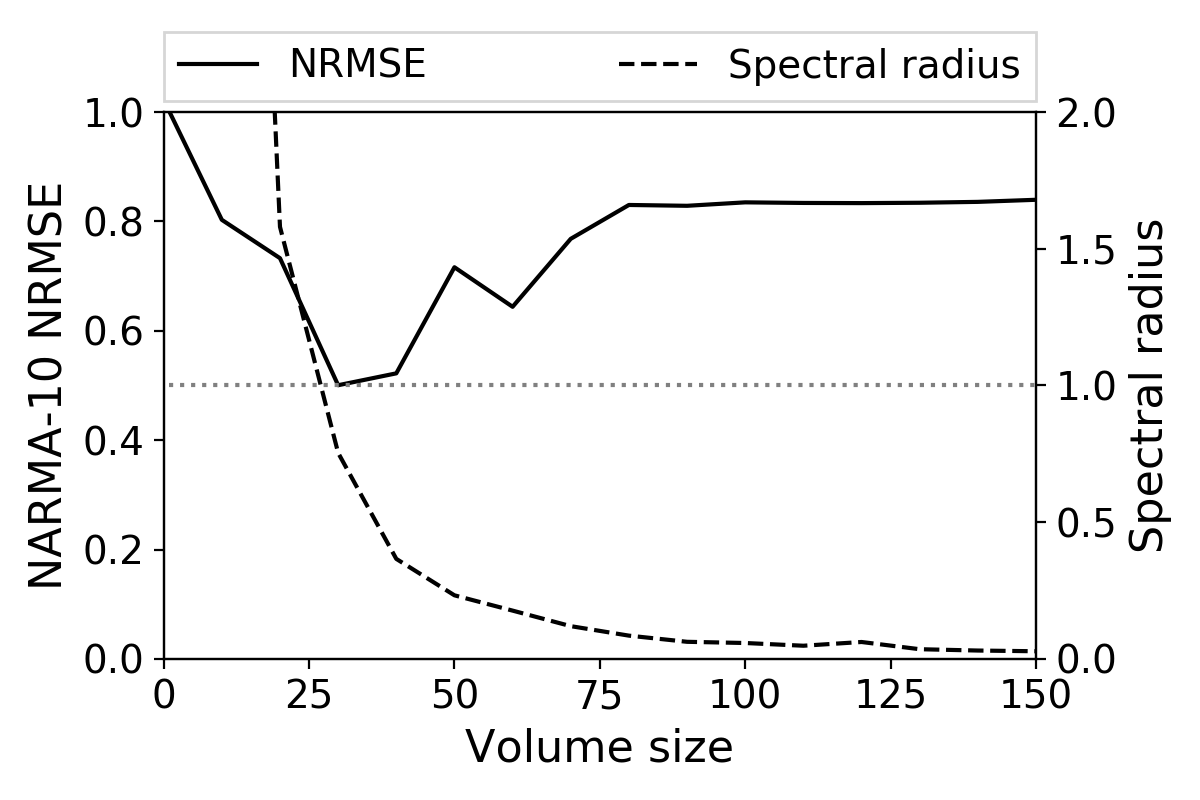
\includegraphics[width=1.0\linewidth]{figures/RGG-volume-size-inv-squared.png}
    \caption{}
    \label{fig:size-graph-volume-b}
  \end{subfigure}
  \caption{
    Spectral radius and performance of generated random geometric graphs of size
$N = 100$, as a function of the size of the underlying volume. Illustrated is
node coupling using two different distance functions: $1/d$ (a) and $1/d^2$ (b).
  }
  \label{fig:size-graph-volume}
\end{figure*}

The results of tuning the underlying volume size $l$ is shown in Figure
\ref{fig:size-graph-volume}. Shown are the results for the distance functions
$1/d$ and $1/d^2$. The plots include both the NRMSE of the network on the
NARMA-10 benchmark, and the resulting spectral radius of its internal reservoir
matrix $\mathbf{W}^{res}$ for the same network.

First, we see that an underlying volume of size $l = 1$ is near useless. The
weights generated by the $1/d$ and $1/d^2$ distance functions are too big, as
expected. The consequence of big weights is that the spectral radius of the
$\mathbf{W}^{res}$ grows too large as well. In fact, the $\tanh$ transfer
function of the internal nodes stays completely saturated throughout the entire
benchmark run.

Next, we see that as the spectral radius of $\mathbf{W}^{res}$ decreases, so
does the benchmark error. It is well-known that a spectral radius that is too
small will cause ordered or fixed-point behavior, and one that is too big may
cause unbounded deviation from initial states. Hence, the valleys seen in Figure
\ref{fig:size-graph-volume}, are equivalent to those seen in early explorations
of the spectral radius property in reservoirs
\cite{verstraeten_experimental_2007}. However, in our case, the spectral radius
is implicitly scaled by stretching the size of the underlying volume in which
the graph is embedded.

Knowledge that stretching the underlying space is equivalent to scaling them
spectral radius of the reservoir is of key interest. In physical contexts, this
means that we can scale the degree of dynamical richness in the reservoir by
moving nodes, or otherwise strengthening or lessening their connectivity. This
conclusion seems obvious, but is of importance for following experiments, as we
can directly scale the spectral radius $\mathbf{W}^{res}$ with confidence that
we could do the same by scaling the metric space.

Performance-wise, spatially constraining ESN reservoirs has caused an increase
in error compared to the non-constrained approach. The best reservoirs, seen at
the bottom of the valley in Figure \ref{fig:size-graph-volume-b}, achieve an
NRMSE around 0.5, with a spectral radius $\boldsymbol{\rho}$ around 0.8. This is
worse than what is achieved using a shift register with perfect memory. There is
thus an indication that spatial restrictions do cause a performance penalty, and
figuring out what is causing this is a main theme of the following sections.

\section{Distance Functions and Memory Capacity}
\label{sec:dist-func}

\subsection{Synopsis}

Before exploring changes to improve upon our RGG model, it is reasonable to
examine the differences between the distance functions we have available, $1/d$,
$1/d^2$, and $1/d^3$. The increasing degree of the inverse of the distance
essentially acts to reduce the neighborhood size $r$. For example, with a
distance function of $1/d^3$, nodes that are distant will have little or no
impact on each other.

Using the knowledge we gained in Section \ref{sec:volume-size}, we now also
directly scale the spectral radius of $\mathbf{W}^{res}$ to 0.9 by multiplying
it by the appropriate scalar.

\subsection{Results and Discussion}

% (TODO): t!
\begin{figure*}[t]
  \centering
  \begin{subfigure}{.49\textwidth}
    \centering
    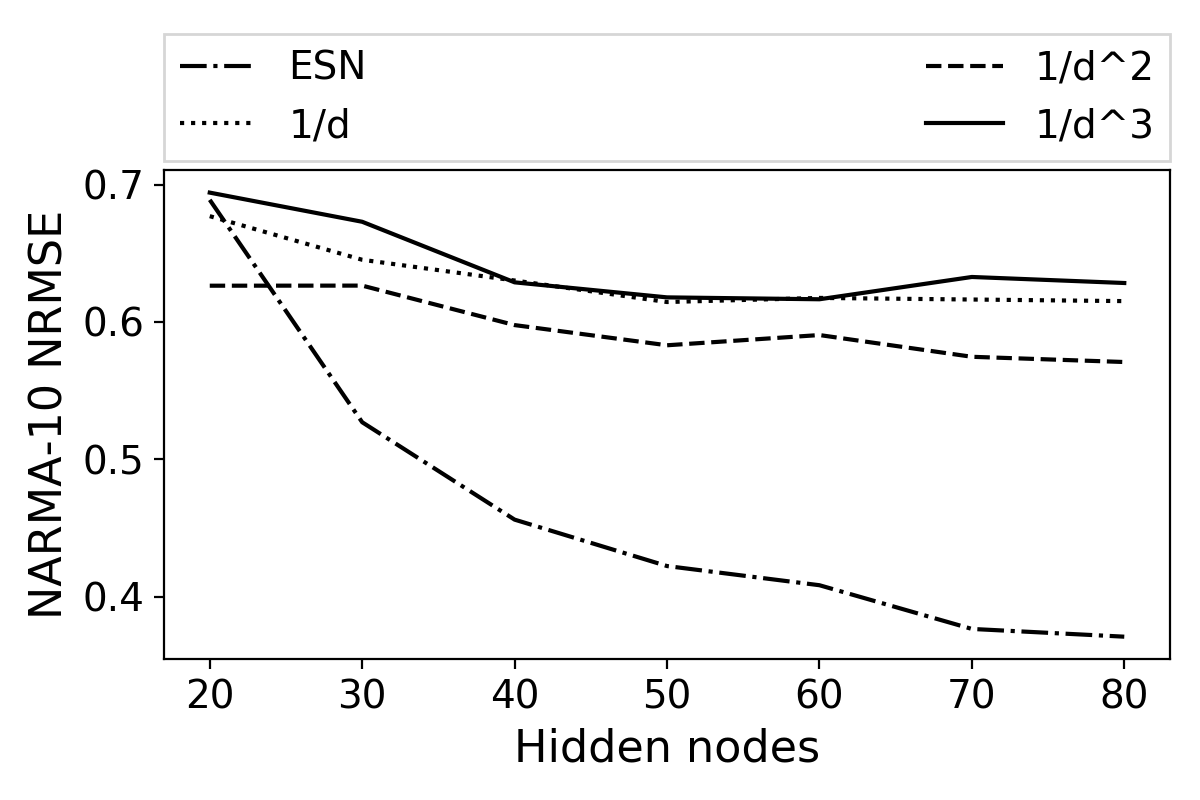
\includegraphics[width=1.0\linewidth]{figures/RGG-dist-performance-mean.png}
    \caption{}
    \label{fig:dist-performance-a}
  \end{subfigure}
  \begin{subfigure}{.49\textwidth}
    \centering
    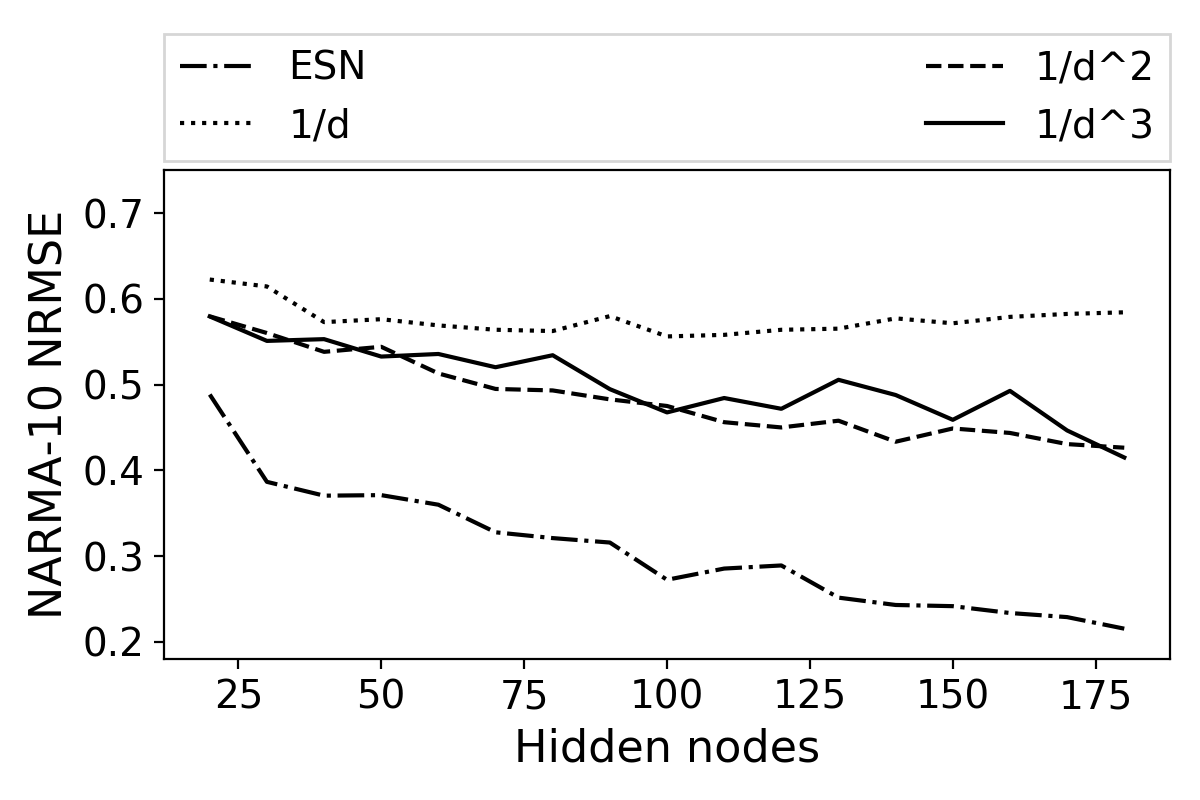
\includegraphics[width=1.0\linewidth]{figures/RGG-dist-performance-min.png}
    \caption{}
    \label{fig:dist-performance-b}
  \end{subfigure}
  \caption{
    NRMSE on the NARMA-10 task with use of different distance functions to
generate connection weights. Plots shown are the mean (a) and minimum (b) error
aggregations over 10 runs per individual parameter setup. Distance functions are
compared to the standard echo state network.
  }
  \label{fig:dist-performance}
\end{figure*}

Figure \ref{fig:dist-performance} compares the performance of the distance
functions to that of default ESNs. Plotted is NARMA-10 NRMSE as a function of
reservoir size. The average over 20 runs, shown in Figure
\ref{fig:dist-performance-a}, shows little noticeable decrease in error for the
distance functions as reservoir size increases. Additionally, it is clear that
there is some degree of variability in the error when using the $1/d^2$ and
$1/d^3$ functions. This notion is strengthened by Figure
\ref{fig:dist-performance-b}, where we see best performances for $1/d$ is about
the same as the mean, while $1/d^2$ and $1/d^3$ show a slight decrease in error
with reservoir size.

% (TODO): t!
\begin{figure*}[t]
  \centering
  \begin{subfigure}{.49\textwidth}
    \centering
    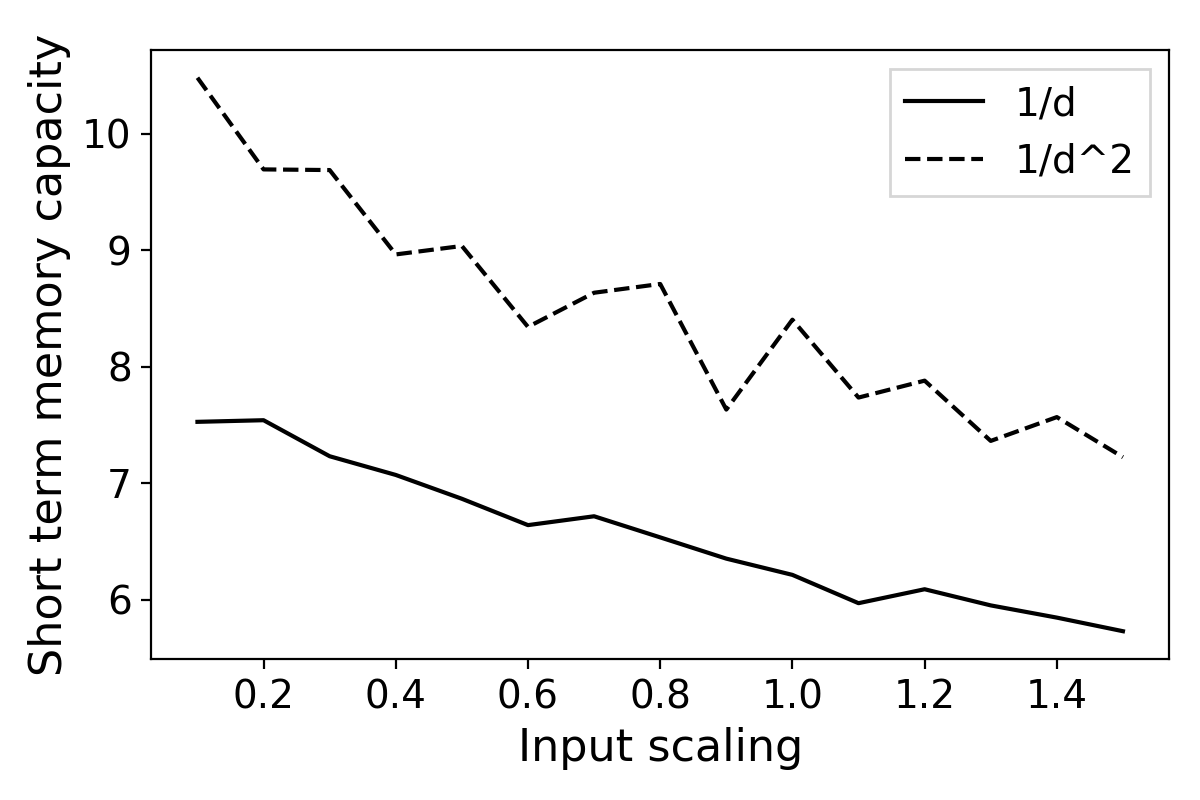
\includegraphics[width=1.0\linewidth]{figures/RGG-dist-mc.png}
    \caption{}
    \label{fig:dist-performance-is-a}
  \end{subfigure}
  \begin{subfigure}{.49\textwidth}
    \centering
    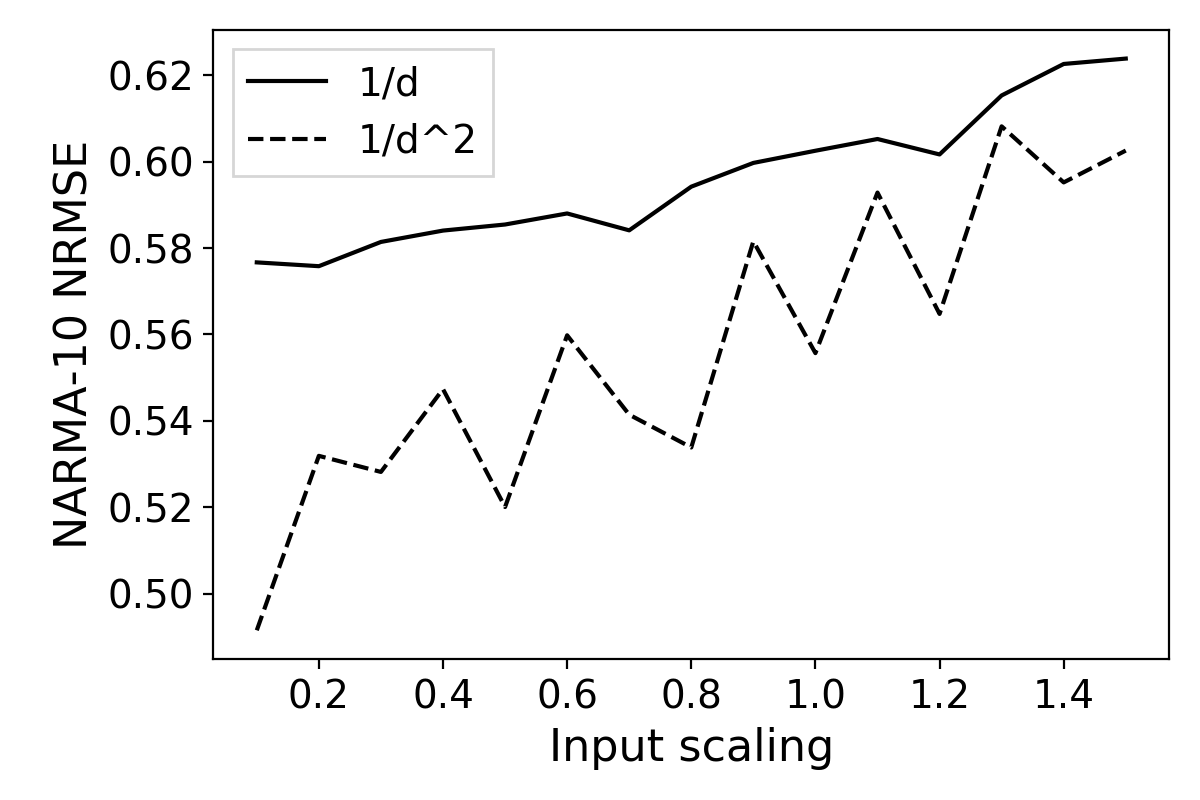
\includegraphics[width=1.0\linewidth]{figures/RGG-dist-performance-is.png}
    \caption{}
    \label{fig:dist-performance-is-b}
  \end{subfigure}
  \caption{
    Effect of input scaling on reservoirs generated as random geometric graphs,
size $N = 80$. There is a correlation between the short-term memory capacity of
the reservoirs (a), and error rates for the NARMA-10 task (b). The distance
function used is $1/d$.
  }
  \label{fig:dist-performance-is}
\end{figure*}

Empirically, we have found that reservoirs that get no significant performance
increase on the NARMA-10 task with an increasing reservoir size, tend to be
limited by memory capacity. The inability of the reservoirs to reach the
performance of a delay line supports this hypothesis. Figure
\ref{fig:dist-performance-is} highlights this, presenting both the short-term
memory capacity and the NARMA-10 NRMSE of reservoirs of size $N = 80$ as a
function of input scaling. As we decrease the input scaling, the memory capacity
increases, and error decreases. This is expected, since determines how nonlinear
the responses of the reservoir are, and there exists a memory-nonlinearity
trade-off, described in Section \ref{ssec:metrics}.

To summarize, we have found that the average performance of our distance
functions seem to hover around similar values. A general trend is that the RGG
model lacks sufficient memory capacity to solve the NARMA-10 task well,
regardless of the distance function used. Memory retention is improved by
lowering the input scaling. Further exploration can also be done by choosing a
single distance function, as our results suggest that they suffer from problems
of a similar nature.

% (TODO): I am not too happy with this section, it is a bit unclear, and might
% not be relevant/needed at all.

\section{Restoring Echo State Network Performance}

\subsection{Synopsis}

Next, we will make changes to the $\mathbf{W}^{res}$ generated with the RGG
model to move its performance close to the ESN. This may seem counter-intuitive,
as we primarily concern ourselves with physical reservoir computing. Making
arbitrary changes to the model generation is not a procedure that will
necessarily translate well to physical substrates and their restrictive
nature. However, we argue that determining the root cause of the difference in
error seen in Figure \ref{fig:dist-performance} will uncover important
properties of reservoir design. In turn, this improves our fundamental
understanding of the paradigm.

In this section, we therefore introduce signedness and directedness to the edges
of the RGG. The signedness of the reservoir is given by some fraction,
e.g. 0.10, such that each edge has a corresponding chance of becoming
negative. Reservoirs are either directed or undirected, where edges in a
directed reservoir have a 50\% chance of going in either direction. Note that
making an edge negative is not the same as reversing the direction, as it simply
means that a node will weight the value of its neighbor negatively.

For these experiments, we use the $1/d$ distance function. In Section
\ref{sec:dist-func} we found this function to give the most stable
results. Although it does not strictly produce the \textit{best} results, we
found the stability to easier to work with when looking for definitive trends in
performance. Similar results were seen with $1/d^2$, though less pronounced. We
also found lowering the input scaling to improve memory capacity, and
experiments in this section will use an input scaling of 0.1

\subsection{Results and Discussion}

% (TODO): t!
\begin{figure*}[t]
  \centering
  \begin{subfigure}{.49\textwidth}
    \centering
    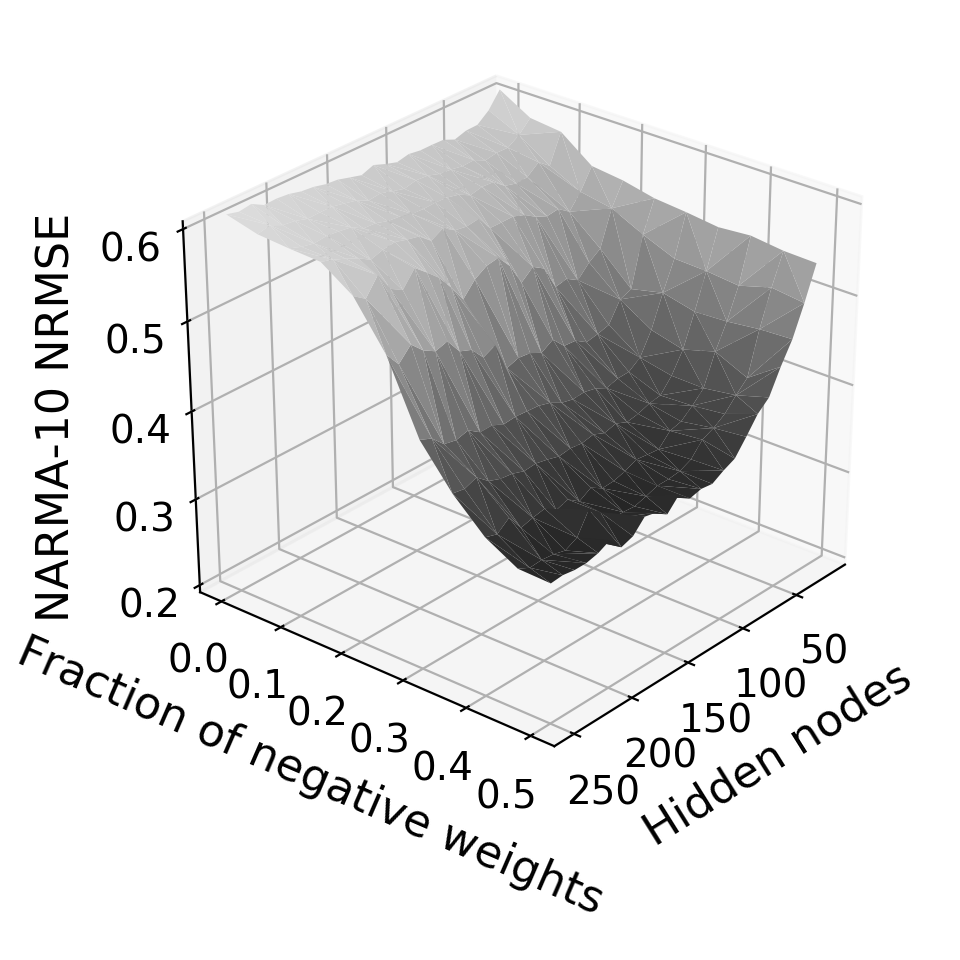
\includegraphics[width=1.0\linewidth]{figures/perf-rest-undir.png}
    \caption{}
    \label{fig:perf-restore-a}
  \end{subfigure}
  \begin{subfigure}{.49\textwidth}
    \centering
    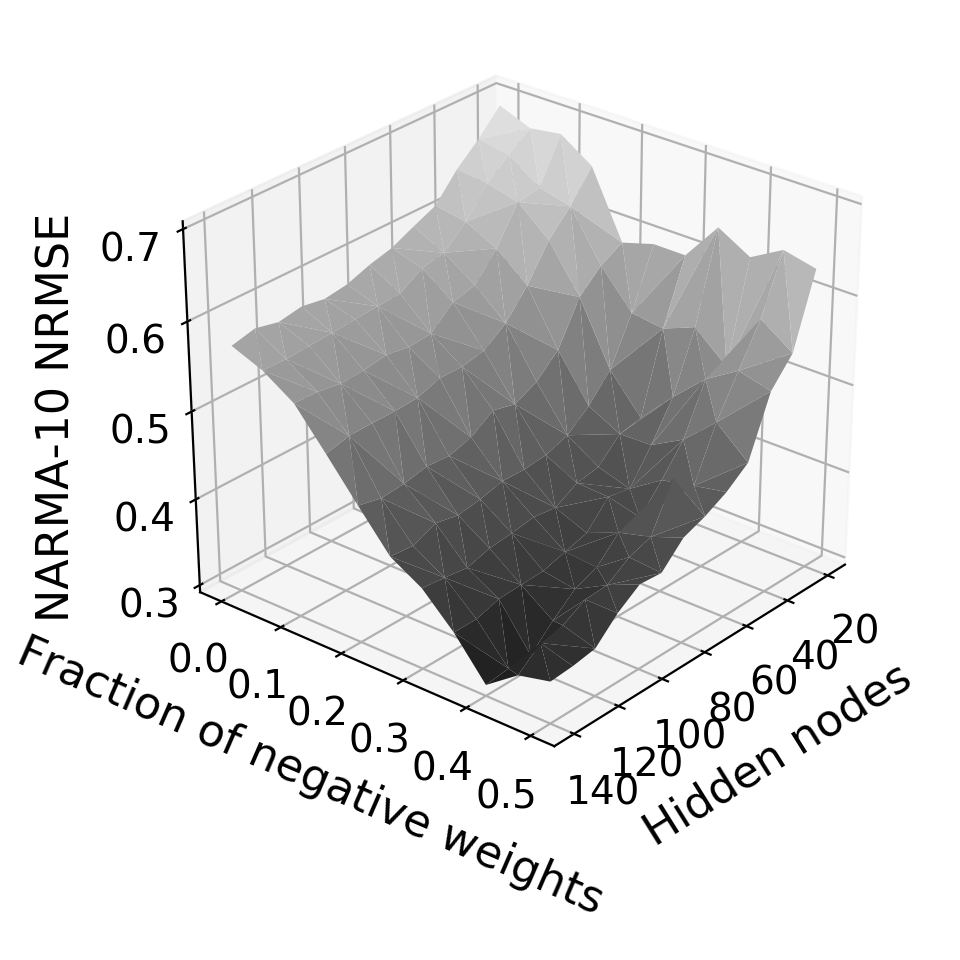
\includegraphics[width=1.0\linewidth]{figures/perf-rest-dir.png}
    \caption{}
    \label{fig:perf-restore-b}
  \end{subfigure}
  \caption{
    Introducing signed weights RGG reservoirs. Results shown are for undirected
(a) and directed (b) reservoirs.
  }
  \label{fig:perf-restore}
\end{figure*}

The impact of introducing signed, directed edges to reservoirs is shown in
Figure \ref{fig:perf-restore}. An increased fraction of signed weights decrease
the benchmark error in all cases, except for very small reservoirs. Moreover,
making the reservoir directed decreases error drastically when the fraction of
negative edges is 0.5. This is particularly true for bigger reservoirs.

Firstly, negative weights discard some of the inherent symmetry of the
network. Although the weight matrix is still symmetric in magnitude, it now
allows for a wider range of node behavior, especially considering that the lower
half of $\tanh$ becomes available. The addition of directed edges makes it clear
that a non-symmetric weight matrix enables richer dynamics, as we move below the
performance of a delay line.

% (TODO): t!
\begin{figure}[t]
  \centering
  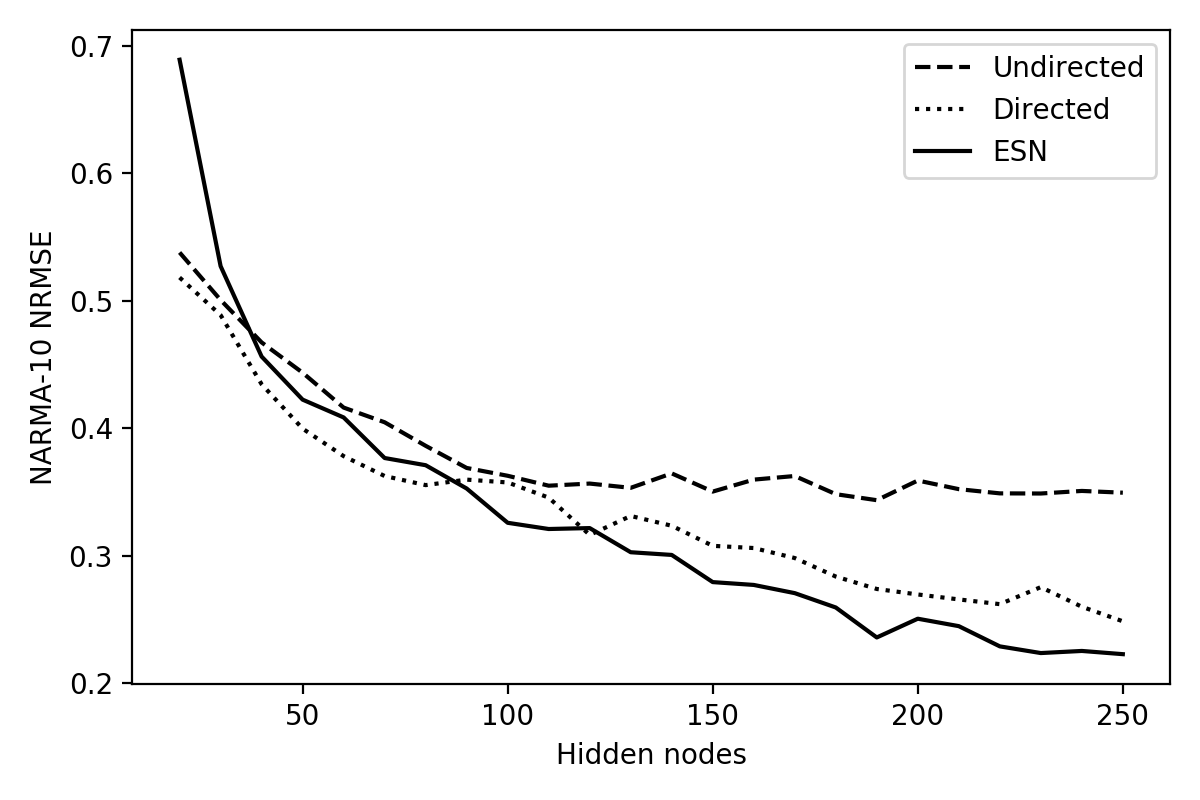
\includegraphics[width=3.5in]{figures/perf-rest-comp.png}
  \caption{
    Comparing RGG reservoirs with signed and directed edges to traditional
ESNs. Both RGG reservoirs have a fraction of negative edges of 0.5.
  }
  \label{fig:perf-rest-comp}
\end{figure}

Figure \ref{fig:perf-rest-comp} compares the performance of these reservoirs
with ESNs. Directed reservoirs with a signed weight fraction of 0.5 perform
comparably to ESNs, and scale similarly with reservoir size. Our interpretation
of this result is that the importance of \textit{flow of information} in
reservoirs should not be understated. It seems that the \textit{structure} of
the reservoir network is crucial, and that \textit{where} information flows is
more important than its magnitude.

A similar conclusion was reached in \cite{mcquillan_role_2019}, where directed
networks were shown to cover a bigger behavior space than their undirected
counterparts.

\section{Reservoir Weight Distribution}

\subsection{Synopsis}

By reintroducing signed and directed edges to the RGG model, it goes back to
resembling traditional ESNs. In fact, the major difference between the RGG model
and ESNs was their distributions of internal reservoir weights. In this section
we make a short comparison between the two.

\subsection{Results and Discussion}

% (TODO): t!
\begin{figure}[t]
  \centering
  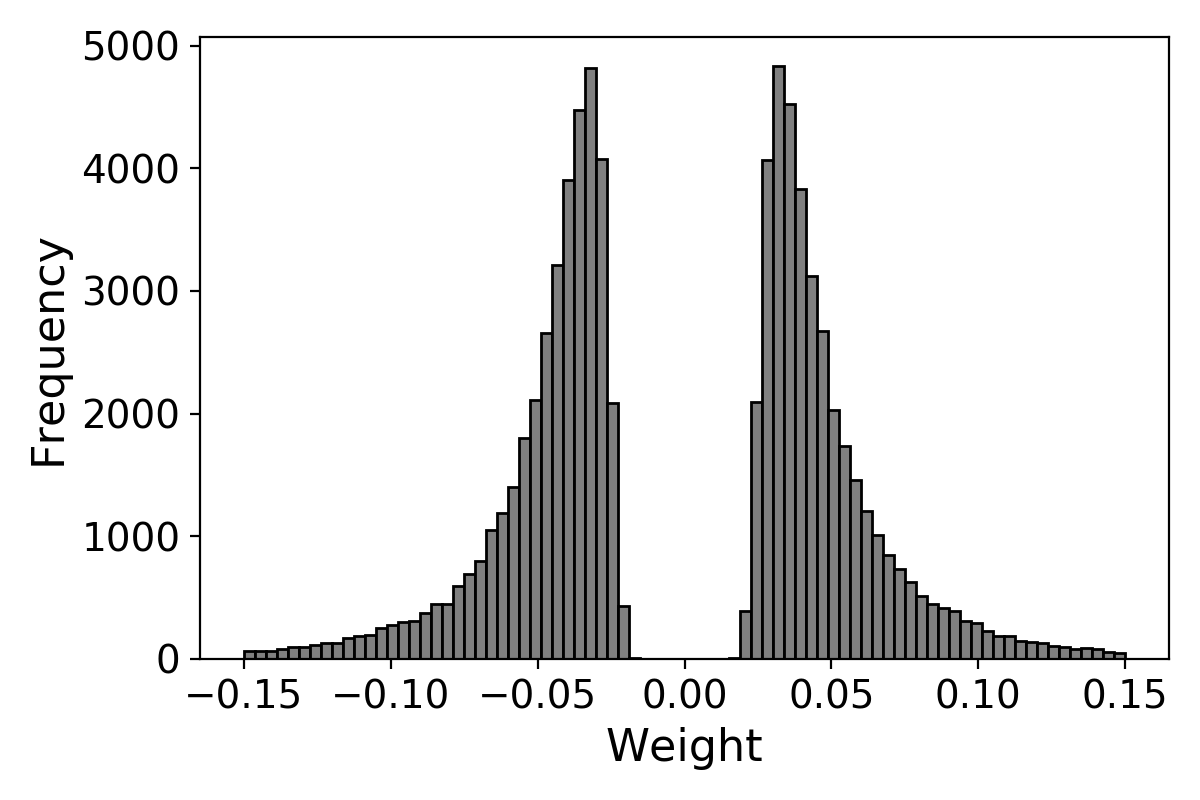
\includegraphics[width=3.5in]{figures/rgg-dist.png}
  \caption{
    Weight distribution of a reservoir with both signed and directed
edges. Zero-elements have been removed, as half of the matrix entries contain
zeroes. The distribution follows the $1/d$ distance function, which incidentally
looks similar to the reciprocal normal distribution.
  }
  \label{fig:rgg-dist}
\end{figure}

The distribution of the internal weights of RGG reservoirs with signed and
directed edges is shown in Figure \ref{fig:rgg-dist}. Three key points are worth
mentioning: (i) the distribution resembles the used distance function $1/d$,
(ii) the distribution is symmetric around zero, due to signed edges, and (iii)
elements of zero magnitude have been removed, as half of $\mathbf{W}^{res}$
contain zero-valued entries due to the directedness of the reservoir.

Distributions commonly proposed to provide ESNs with good performance include a
symmetrical uniform distribution, or a normal distribution centered around zero
\cite{montavon_practical_2012}. We end up with a symmetric distribution
resulting from the distance function $1/d$, a distribution resembling the
inverse Gaussian distribution. This distribution has, to our knowledge, not been
used in previous experiments.

Finally, we mention that the dimensionality of the underlying metric space of
the RGG plays a small role in the performance of the resulting
reservoirs. Changing the dimensionality will simply shift the weight
distribution slightly, causing little change in performance.

\section{Conclusions}

\textcolor{red}{
  The goal of.. was to..
}

\textcolor{red}{
  We have investigated imposing the simplest type of spatial restriction onto
echo state networks, and found that they by default will worsen significantly by
default. Care must be taken to ensure that the spacing between nodes will result
in node interactions that induce reservoir dynamics that are suitable for the
task at hand. This is especially important in physical reservoir computing where
the distance between nodes decides their coupling, and it can not be changed
after-the-fact.
}

% (TODO): Look more into this if found _why_ this causes this improvement,
% concretely.
\textcolor{red}{
  Further we investigated why the spatial restrictions worsened the networks
significantly, arriving at some interesting conclusions regarding flow of
information.
}

\textcolor{red}{
  Highlight the important discoveries in this chapter that lead well into the
next chapter. We would like to highlight two key discoveries: \textbf{(1)} the
fact that there are other weighting distribution schemes that work just as well
as uniform and normal, here we have discovered something that resembles the
reciprocal normal distribution using $1/d$, $1/d^2$ etc. And \textbf{(2)} that
reservoirs worsen significantly if there is no inherent flow of information,
which we in this case restored by introducing signedness and directedness to the
reservoir edges. These discoveries are important springboards into the next
chapter.
}


%%% Local Variables:
%%% mode: latex
%%% TeX-master: "../thesis"
%%% End:

\chapter{Experiments: Lattices}
\label{ch:regular-tilings}

% (TODO): Overall: standard deviations.

% (TODO): Remember to always specify specifics of experiment setups for all
% experiments

% (TODO): t!
\begin{figure*}[t]
  \centering
  \begin{subfigure}{.32\textwidth}
    \centering
    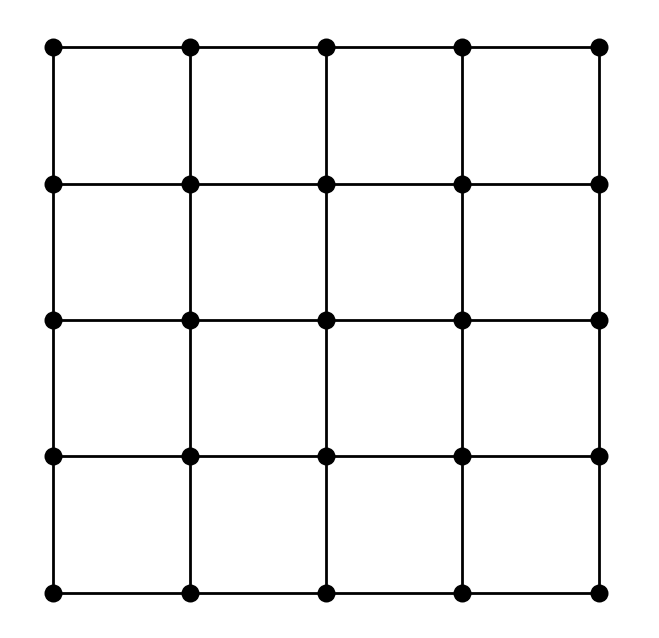
\includegraphics[width=1.0\linewidth]{figures/square.png}
    \label{fig:rt-square}
  \end{subfigure}
  \begin{subfigure}{.32\textwidth}
    \centering
    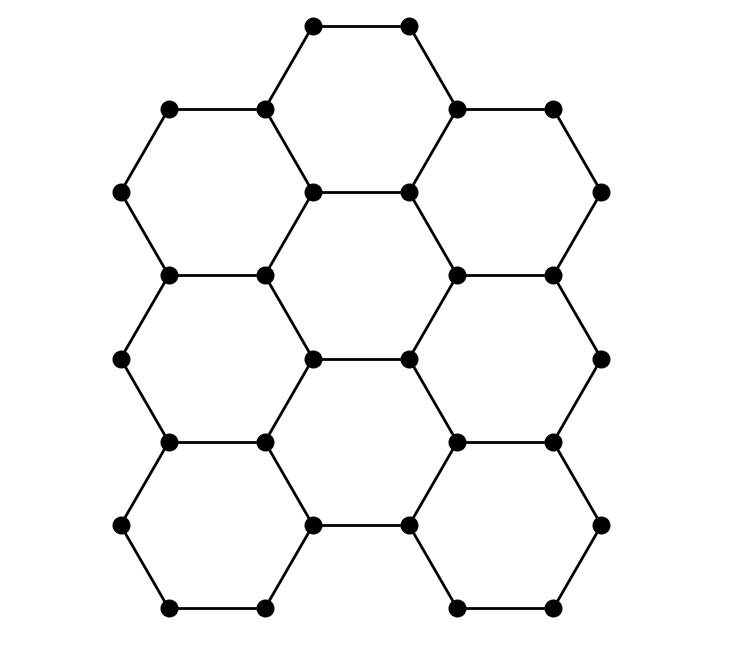
\includegraphics[width=1.0\linewidth]{figures/hex.png}
    \label{fig:rt-hex}
  \end{subfigure}
  \begin{subfigure}{.32\textwidth}
    \centering
    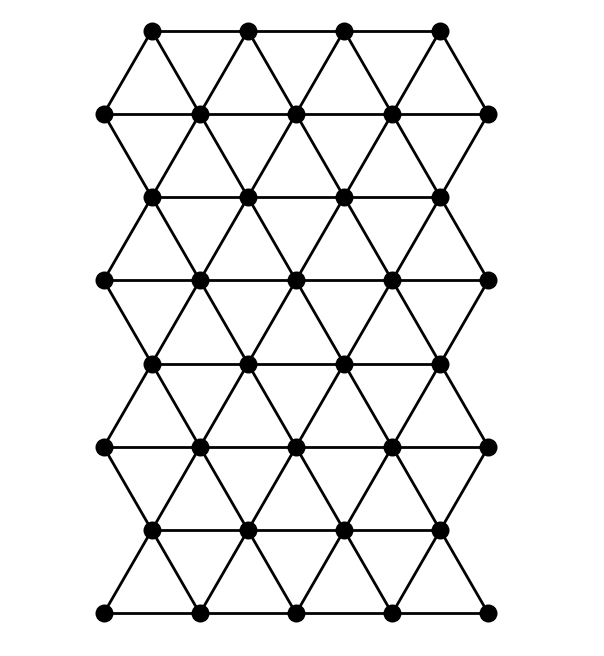
\includegraphics[width=1.0\linewidth]{figures/triangular.png}
    \label{fig:rt-tri}
  \end{subfigure}
  \caption{
    Types of lattices investigated for their quality as reservoir
topologies. Investigated tilings include square (a), hexagonal (b), and
triangular (c).
  }
  \label{fig:regular-tilings}
\end{figure*}

Lattice models are common in computational physics
\cite{lavis_equilibrium_2015}. Understanding important models of computational
physics in reservoir contexts is thus crucial to advance physical RC
methodology. For example, the Ising model with dipole moments of atomic spins
\cite{jensen_computation_2018}, spin-torque oscillator arrays
\cite{tsunegi_physical_2019}, and the Ginzburg-Landau equation
\cite{opala_neuromorphic_2019}, describe systems that are employed on a
two-dimensional lattice, and have been used in reservoir settings. In this
chapter, we therefore investigate lattice networks as more realistic models of
physical reservoirs.

We explore the properties that lattice graphs exhibit as reservoirs by
structuring internal nodes in this manner. Lattice graphs may be embedded in
Euclidean space to form regular tilings, of which there three in two-dimensional
space: square, hexagonal and triangular, which are all depicted in Figure
\ref{fig:regular-tilings}. Other, more complicated tiling schemes
exist. Semiregular, often called uniform, tilings are created using two or more
faces. However, complicated grids are left outside the scope of this thesis, as
our primary focus is the fundamental applicability of lattice layouts, not
comparing the performance between them.

Reservoirs are created by replacing the reservoirs of ESN models with the
adjacency matrix generated for lattice models. For each experiment,
$\mathbf{W}^{res}$ is then scaled to a spectral radius of 0.9, as this is
equivalent to scaling the coupling, or spacing, between nodes in a physical
system. Beyond this, our reservoir model remains the same as that of the ESN.

\section{Reservoir Quality of Lattices}
\label{sec:lattice-quality}

\subsection{Synopsis}

First, we evaluate the default quality of lattice reservoirs with the NARMA-10
benchmark. Reservoirs are generated by embedding internal nodes in a metric
space, much like in Figure \ref{fig:regular-tilings}, and connecting neighboring
pairs with an edge of unit length. Nodes along the edges are not connected to
the opposite side of the lattice, making the lattice aperiodic. Lastly, unit
weight of all edges are scaled by the appropriate scalar to allow a spectral
radius of 0.9.

\subsection{Results and Discussion}

% (TODO): t!
\begin{figure}[t]
  \centering
  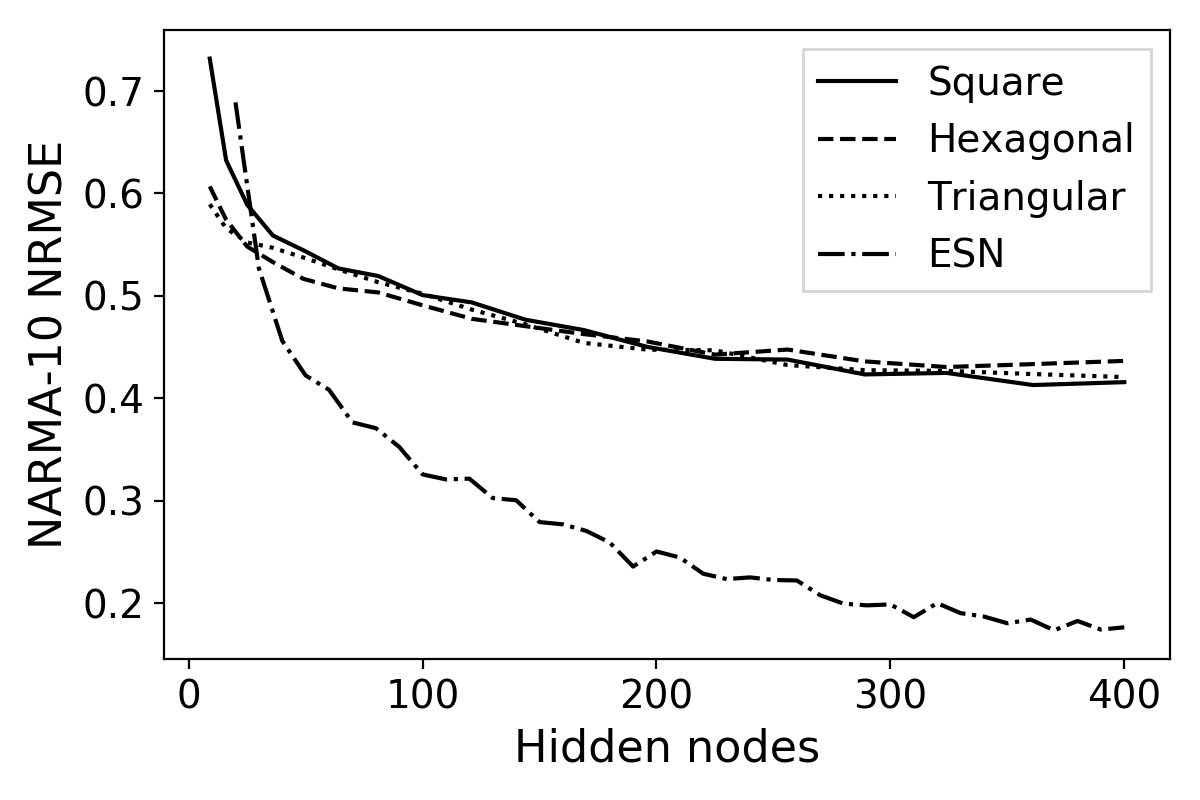
\includegraphics[width=3.5in]{figures/regular-tilings-performance.png}
  \caption{
    NARMA-10 NRMSE of square, hexagonal, and triangular regular tilings as
reservoir topologies.
  }
  \label{fig:rt-performance}
\end{figure}

Figure \ref{fig:rt-performance} shows how reservoir error scales with reservoir
size. We see that restricting reservoir topologies to lattice structures results
in a significant performance penalty. Additionally, little difference is seen
between the three types of tilings.

% (TODO): t!
\begin{figure*}[t]
  \centering
  \begin{subfigure}{.32\textwidth}
    \centering
    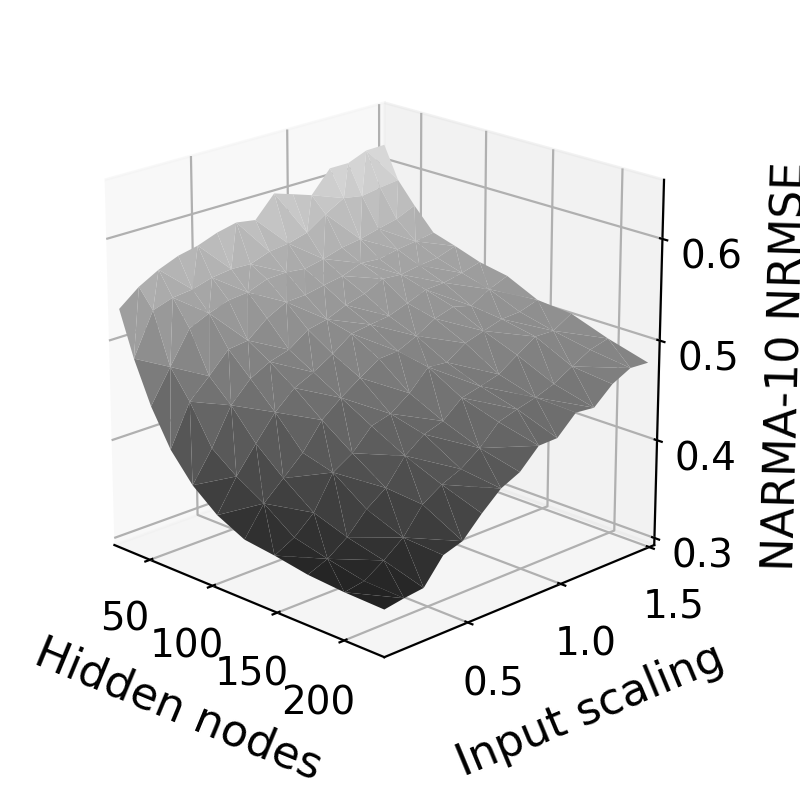
\includegraphics[width=1.0\linewidth]{figures/regular-tilings-performance-is-sq.png}
    \caption{}
    \label{fig:rt-is-square}
  \end{subfigure}
  \begin{subfigure}{.32\textwidth}
    \centering
    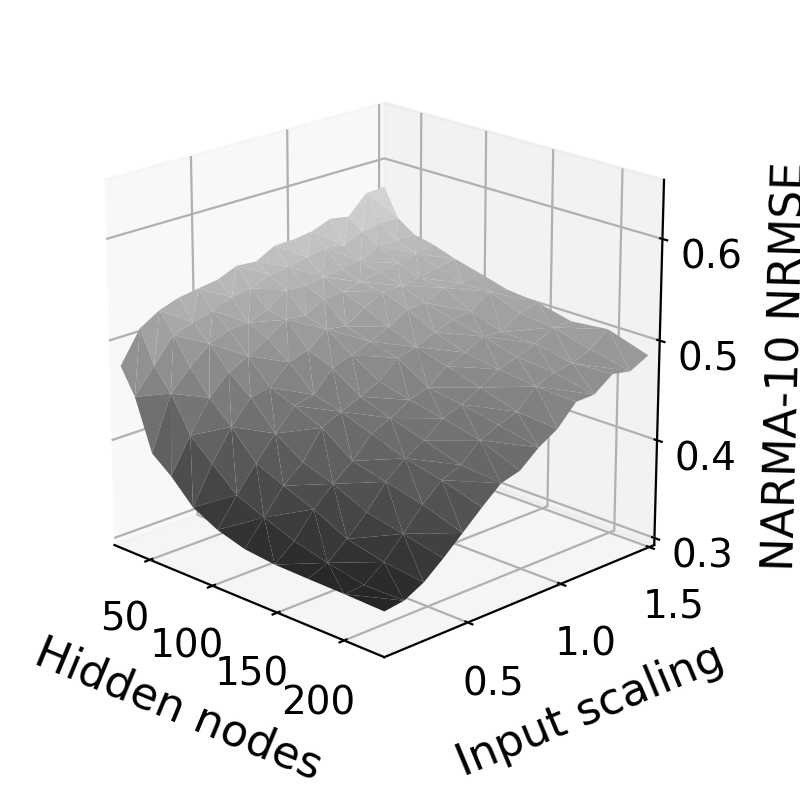
\includegraphics[width=1.0\linewidth]{figures/regular-tilings-performance-is-hex.png}
    \caption{}
    \label{fig:rt-is-hex}
  \end{subfigure}
  \begin{subfigure}{.32\textwidth}
    \centering
    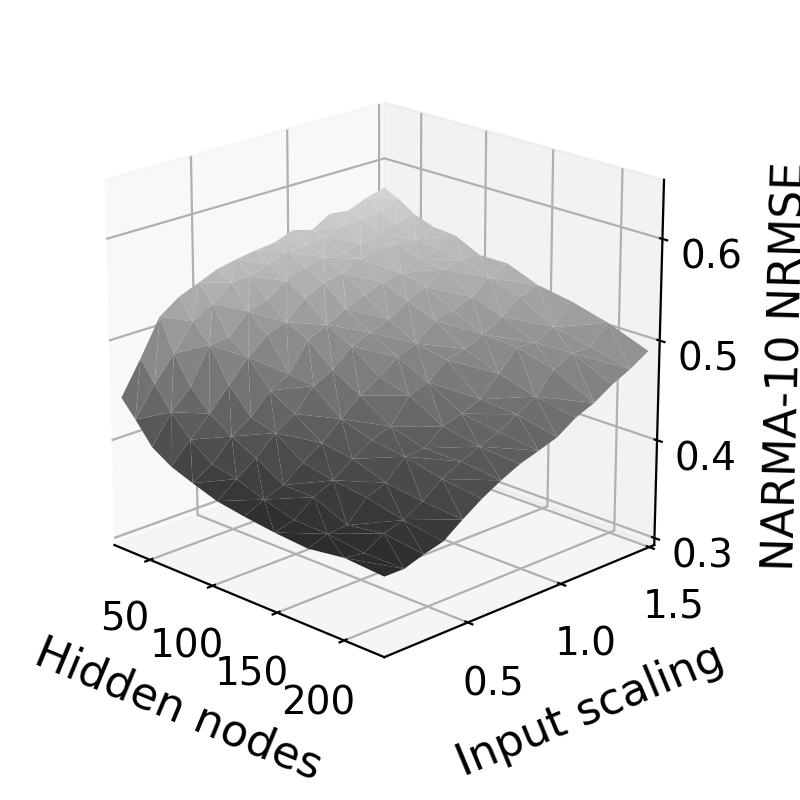
\includegraphics[width=1.0\linewidth]{figures/regular-tilings-performance-is-tri.png}
    \caption{}
    \label{fi:rt-is-tri}
  \end{subfigure}
  \caption{
    Regular tilings investigated for their quality as reservoir topologies, here
as a function of reservoir size and input scaling. Investigated topologies
include square (a), hexagonal (b), and triangular (c) regular tilings.
  }
  \label{fig:rt-performance-is}
\end{figure*}

In Section \ref{sec:dist-func}, it was discovered that reservoirs modeling
random geometric graphs exhibited low memory retention. The symptoms are similar
here: the lattice reservoirs perform worse than a delay line would, and only
perform marginally better with an increasing size. Figure
\ref{fig:rt-performance-is} illustrates the effect of scaling the magnitude of
the input. Again, we see clearly see reservoirs favoring low input scaling
values.

We interpret these results to indicate that the structure imposed by an
undirected lattice shifts the point of criticality described in
\ref{sec:criticality}. When input scaling is lessened such that the required
memory capacity for the benchmark task is reached, the error diminishes rapidly,
and the existing reservoir dynamics work as intended.

Curiously, the NRMSE differs only slightly between the three types of
lattice. It seems that it is the overall lattice structure that is important,
not the specific type of tiling implementing it. We therefore argue that the
different tilings, which in practice dictate the amount of incident edges per
vertex, work mostly as minor tuning parameters. The idea that overall structure
is important is in accordance with our findings in \ref{sec:restore}, concluding
that \textit{how information flows} in the network is vital.

Input scaling decreased the benchmark error of lattice reservoirs, but the best
performing networks of Figure \ref{fig:rt-performance-is} are not quite
comparable to the ESN. For example, square grid reservoirs of size 200 benchmark
a mean NRMSE of around 0.35, while corresponding ESNs average around 0.25.

Overall, it is interesting that undirected lattice reservoirs perform as well as
they do. On the other hand, the distribution of the input weights are drawn from
a uniform distribution in the interval [-0.5, 0.5], letting internal nodes see
varying representations of the input signal. As physical substrates may differ
in the input schemes they offer, the input scheme will be further investigated
in the next section.

To summarize, we have in this section found undirected lattice reservoirs to
provide promising results. A key discovery of Chapter \ref{ch:rgg} is the
importance of a directed flow of information, and whether directedness also
improves lattice models is the topic of the next section.

\section{Lattices with Directed Edges}
\label{sec:lat-dir-edge}

\subsection{Synopsis}

% (TODO): t!
\begin{figure*}[t]
  \centering
  \begin{subfigure}{.40\textwidth}
    \centering
    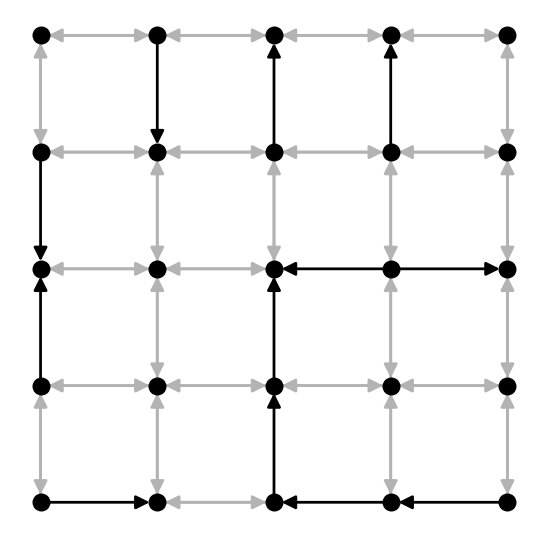
\includegraphics[width=1.0\linewidth]{figures/dir_lattice_025.png}
    \caption{}
    \label{fig:dir-lattice-a}
  \end{subfigure}
  \hspace{25pt}
  \begin{subfigure}{.40\textwidth}
    \centering
    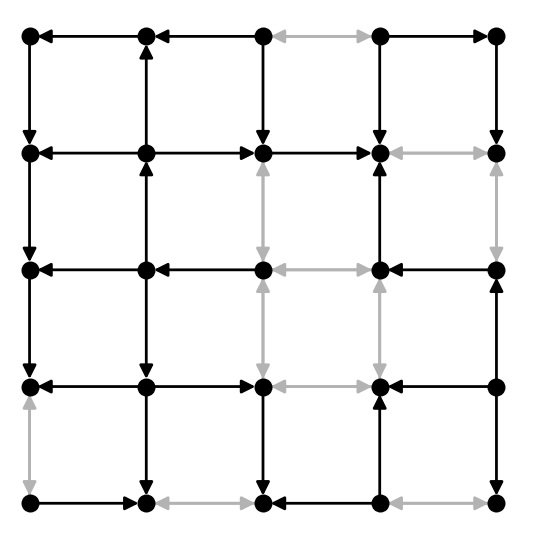
\includegraphics[width=1.0\linewidth]{figures/dir_lattice_075.png}
    \caption{}
    \label{fig:dir-lattice-b}
  \end{subfigure}
  \caption{
    Example square grids where 25\% (a) and 75\% (b) of the undirected edges are
made directed.
  }
  \label{fig:dir-lattice}
\end{figure*}

One of the key discoveries of Chapter \ref{ch:rgg} is that directed edges
improve performance significantly in random geometric graph reservoirs. It is of
interest to repeat this experiment with lattice reservoirs, especially since
information flow is so clearly visible in a lattice structure. We modify the
generated lattice graphs generated in previous sections of this chapter to have
a fraction of directed edges. Figure \ref{fig:dir-lattice} illustrates the
concept for square lattices, where 25\% and 75\% of the edges of the two
lattices, respectively, have been directed. The directed reservoir edges have a
50\% chance of going in either direction.

\subsection{Results and Discussion}

% (TODO): t!
\begin{figure*}[t]
  \centering
  \begin{subfigure}{.32\textwidth}
    \centering
    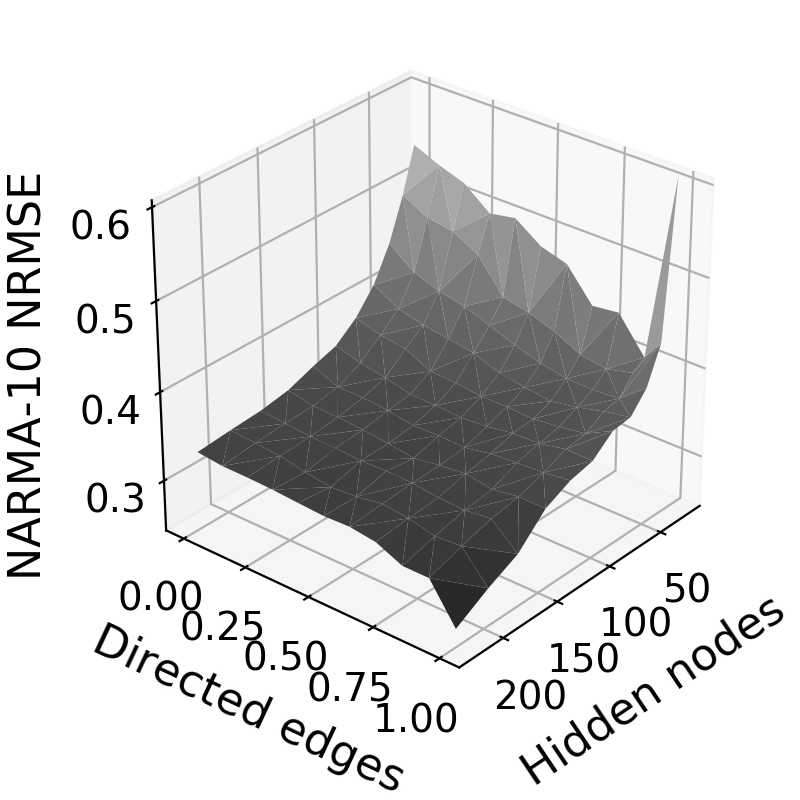
\includegraphics[width=1.0\linewidth]{figures/rt-dir-perf-sq.png}
    \caption{}
    \label{fig:rt-dir-perf-trisurf-sq}
  \end{subfigure}
  \begin{subfigure}{.32\textwidth}
    \centering
    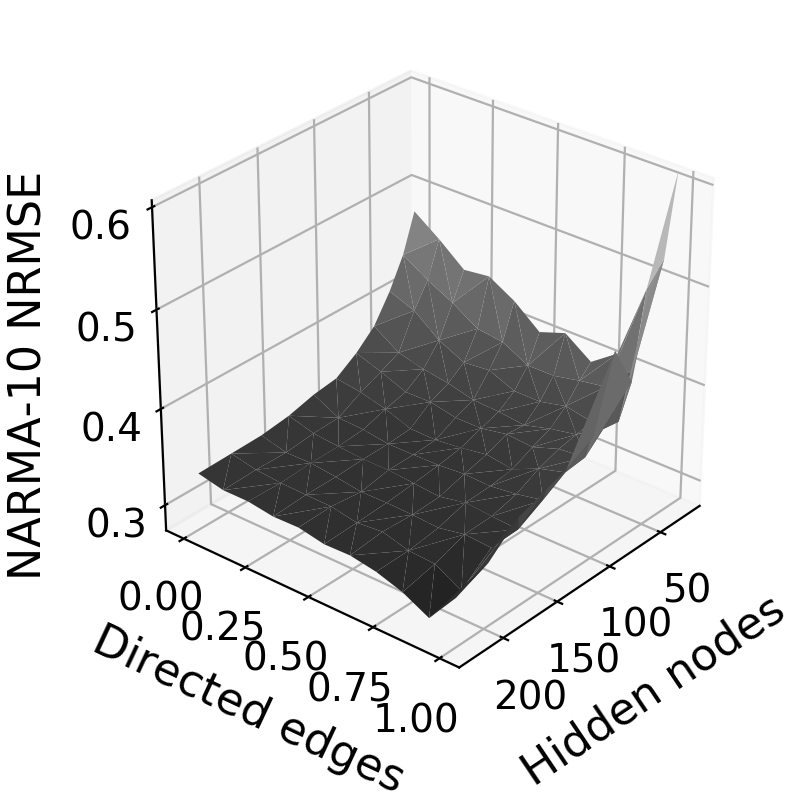
\includegraphics[width=1.0\linewidth]{figures/rt-dir-perf-hex.png}
    \caption{}
    \label{fig:rt-dir-perf-trisurf-hex}
  \end{subfigure}
  \begin{subfigure}{.32\textwidth}
    \centering
    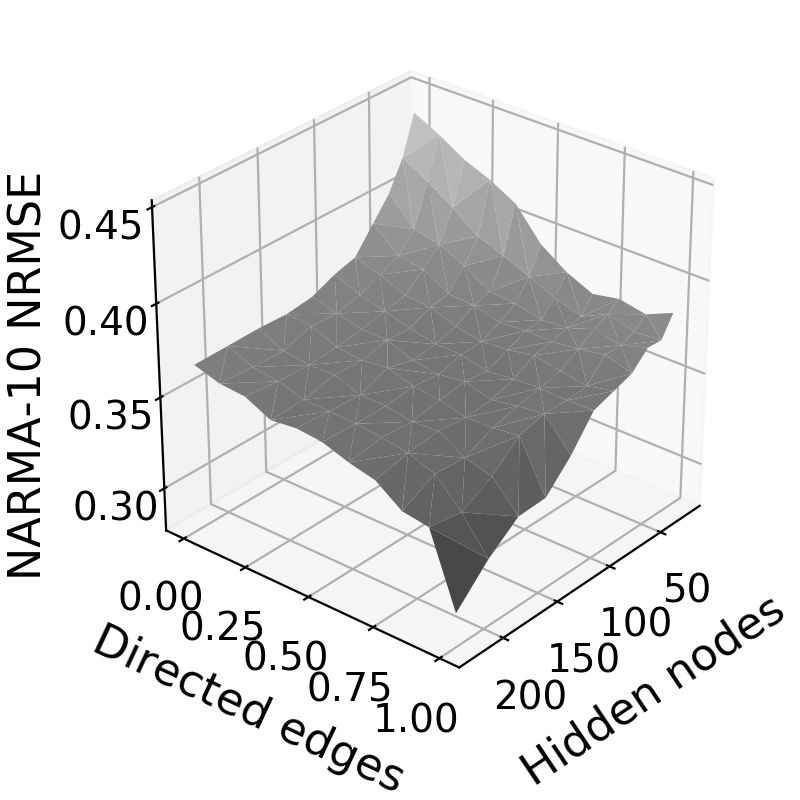
\includegraphics[width=1.0\linewidth]{figures/rt-dir-perf-tri.png}
    \caption{}
    \label{fig:rt-dir-perf-trisurf-tri}
  \end{subfigure}
  \caption{
    Benchmark error as a function of reservoir size and directedness. The
fraction of directed edges determines the amount of edges that are left
bidirectional, explained by Figure \protect\ref{fig:dir-lattice}. Shown are
results for square (a), hexagonal (b) and triangular (c) lattices.
  }
  \label{fig:rt-dir-perf-trisurf}

  \centering
  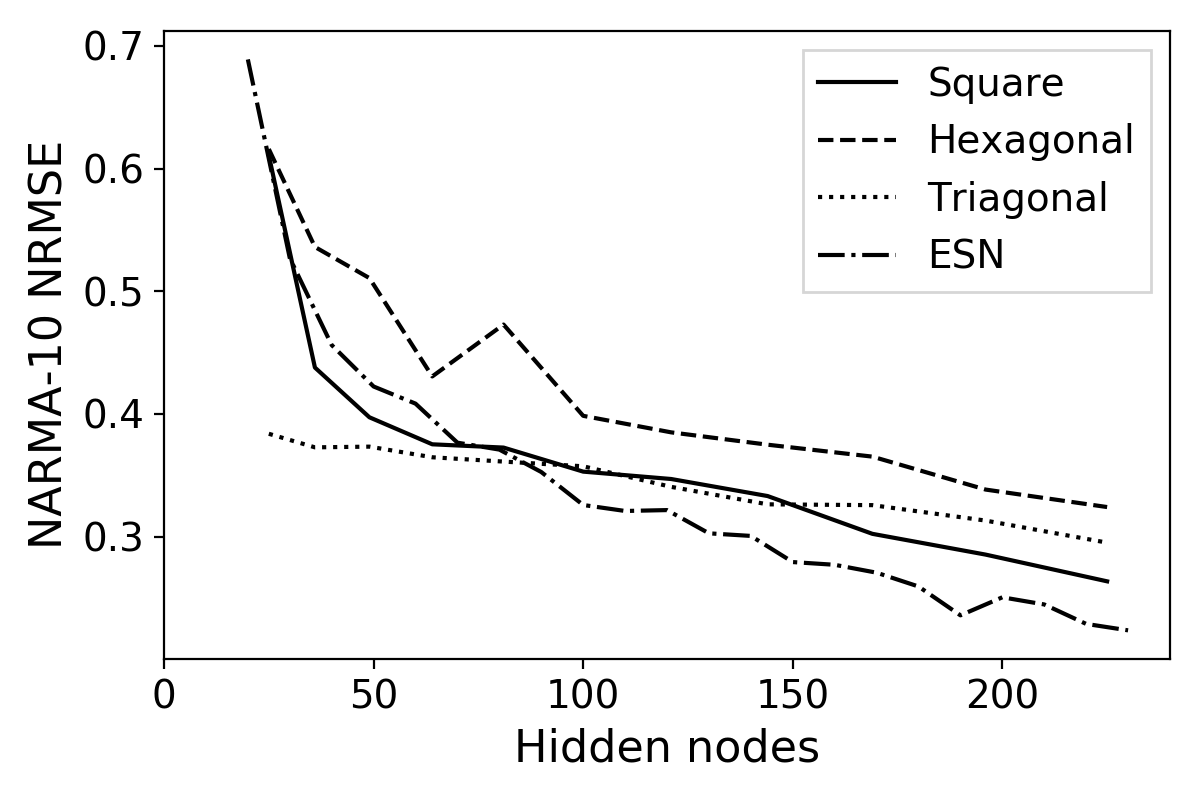
\includegraphics[width=3.5in]{figures/rt-dir-perf.png}
  \caption{
    Benchmark error as a function of size for directed lattice reservoirs. All
reservoirs are fully directed, and the direction of each edge is decided by an
unbiased coin toss.
  }
  \label{fig:rt-dir-perf}
\end{figure*}

Figure \ref{fig:rt-dir-perf-trisurf} presents the results of introducing a
fraction of directed edges to lattice reservoirs. Most reservoirs show reduced
error rates with increasing fractions of directed edges.

A small exception is visible for very small square and hexagonal reservoirs,
where a fully directed reservoir may degrade if the edges align in an
insufficient manner. Nodes in triangular reservoirs have six incident edges, as
opposed to the three and four of square and hexagonal, thus giving a smaller
chance of insufficient reservoirs appearing. Note that this problem disappears
with bigger reservoirs. This compelling result indicates that our method of
generating directed edges guarantees good reservoirs as their sizes increase --
one does not need to ``get lucky'' with directions.

Convincing improvements are exhibited once reservoirs become fully directed and
sufficiently big, which is especially visible at the sudden drops at the closest
points of the surface areas. The drops are only sudden when compared to
reservoirs of a lower fraction of directed edges. We plot the cross section of
the surface areas at full directedness in Figure \ref{fig:rt-dir-perf}, showing
that the error rates keep decreasing with increased reservoir size. This is
again in stark contrast to their undirected counterparts, which in Section
\ref{sec:lattice-quality}, and also previous in Section \ref{sec:restore} only
perform marginally better as reservoir size is increased.

\begin{figure}
  \centering
  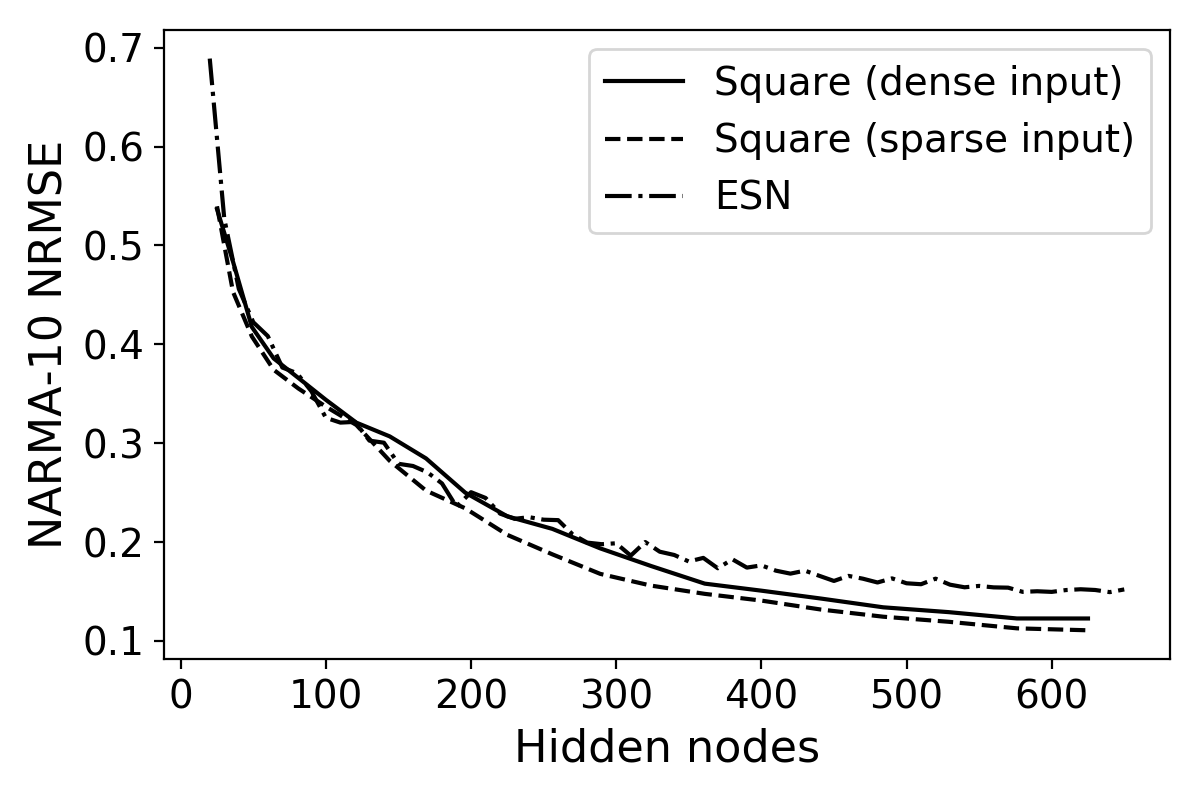
\includegraphics[width=3.5in]{figures/rt-performance-big.png}
  \caption{
    NRMSE of square lattice reservoirs with global, fixed input schemes compared
to standard ESNs. With the sparse input scheme only 50\% of the hidden nodes see
the input.
  }
  \label{fig:rt-performance-big}
\end{figure}

Thus, twice we have found directed edges to improve reservoir performance
significantly, once in random geometric graph reservoirs in Section
\ref{sec:restore}, and now again in lattices. Despite this, lattice reservoirs
still perform slightly worse than ESN.

In the project preceding this thesis, it was found that a global input scheme,
i.e. an input scheme where every input weight is set to 1 and then scaled, works
with ESNs given appropriate scaling \cite{aven_exploring_2019}. This simple
input scheme is relevant to physical RC, given physical substrates in which
every node is forced to see the same input. Results from using this input scheme
with square grids are shown in Figure \ref{fig:rt-performance-big}.

It is abundantly clear that the global input scheme works well with the square
lattice. In fact, it scales even better with reservoir size than the regular
ESNs used in our experiments. Additionally, we have also included error rates
for a square grid with a sparser input scheme in which only 50\% of the hidden
nodes see the input. These networks marginally improve even further upon the
performance of square lattices.

% (TODO): t!
\begin{table}[t]
  \centering
  \begin{center}
    \caption{
      Simplicity of the weighting scheme of square grids. Square grid reservoirs
contain a single unique magnitude for input and reservoir weights. Displayed
values are given as an average across 20 experiment runs (std. dev.).
    }
    \label{tab:sq-global-input}
    \begin{tabular}{c c c c c}
      \hline
      \thead{Reservoir type} & \thead{Hidden \\ nodes} & \thead{Unique \\ input weights} & \thead{Unique \\ reservoir weights} & \thead{NARMA-10 \\ NRMSE} \\
      \hline
      \rule{0pt}{2.5ex}Square grid & 100 & 1 & 1 & 0.346 (0.019) \\
      Square grid & 225 & 1 & 1 & 0.245 (0.022) \\
      Square grid & 400 & 1 & 1 & 0.168 (0.009) \\
      \rule{0pt}{3ex}ESN & 100 & 100 & 997 (26) & 0.388 (0.019) \\
      ESN & 225 & 225 & 5098 (74) & 0.282 (0.019) \\
      ESN & 400 & 400 & 16070 (113) & 0.215 (0.021)\rule[-1ex]{0pt}{0pt} \\
      \hline
    \end{tabular}
  \end{center}
\end{table}

Table \ref{tab:sq-global-input} shows the simplicity of the square grids used in
Figure \ref{fig:rt-performance-big}. The input of the entire reservoir is
decided by a single scalar. Furthermore, there is still only a single unique
magnitude used for reservoir weights in $\mathbf{W}^{res}$, which is determined
by the spacing of nodes.

Simple cyclic reservoirs (SCR) use topology in a similar manner to use a
deterministic weighting scheme \cite{rodan_minimum_2011}. Units in SCRs are
organized in a cycle, with a single unique weight magnitude. All input
connections have the same absolute weight value, but the sign is determined by
means of an unbiased coin. The intention with SCR is to remove stochasticity in
reservoir generation. With square lattices a similar strategy is
employed. However, we do not use a stochastic scheme of generating signed input
values, but instead generate the flow of information in this manner. This leaves
an opportunity to study the structures that are generated, allowing us to peer
into the apparent black box of the ESN, as we shall see in Section
\ref{sec:shrink-grow}.

% (TODO): t!
\begin{figure*}[t]
  \centering
  \begin{subfigure}{.49\textwidth}
    \centering
    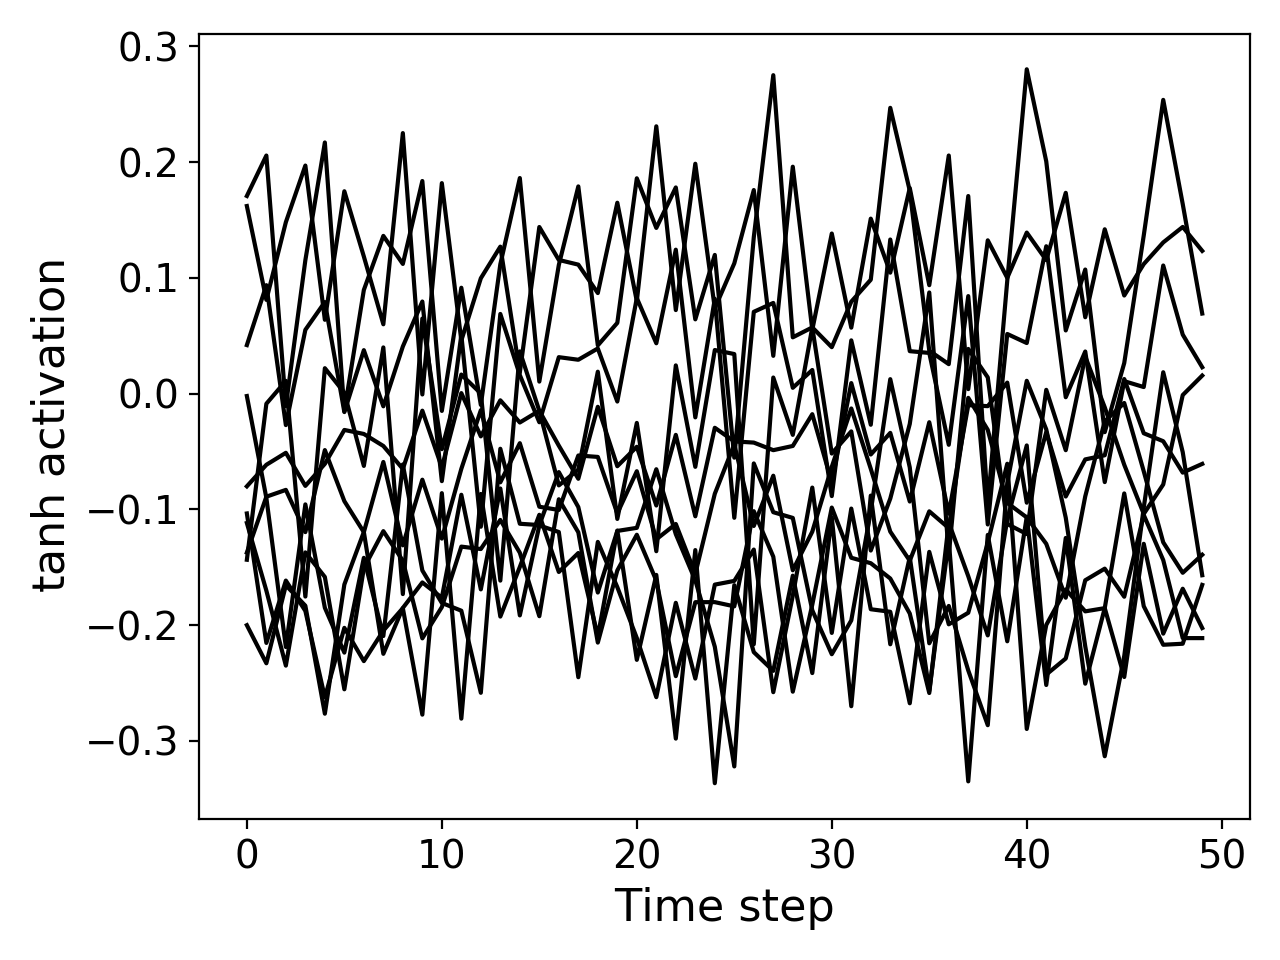
\includegraphics[width=1.0\linewidth]{figures/esn-activations.png}
    \caption{}
    \label{fig:activations-a}
  \end{subfigure}
  \begin{subfigure}{.49\textwidth}
    \centering
    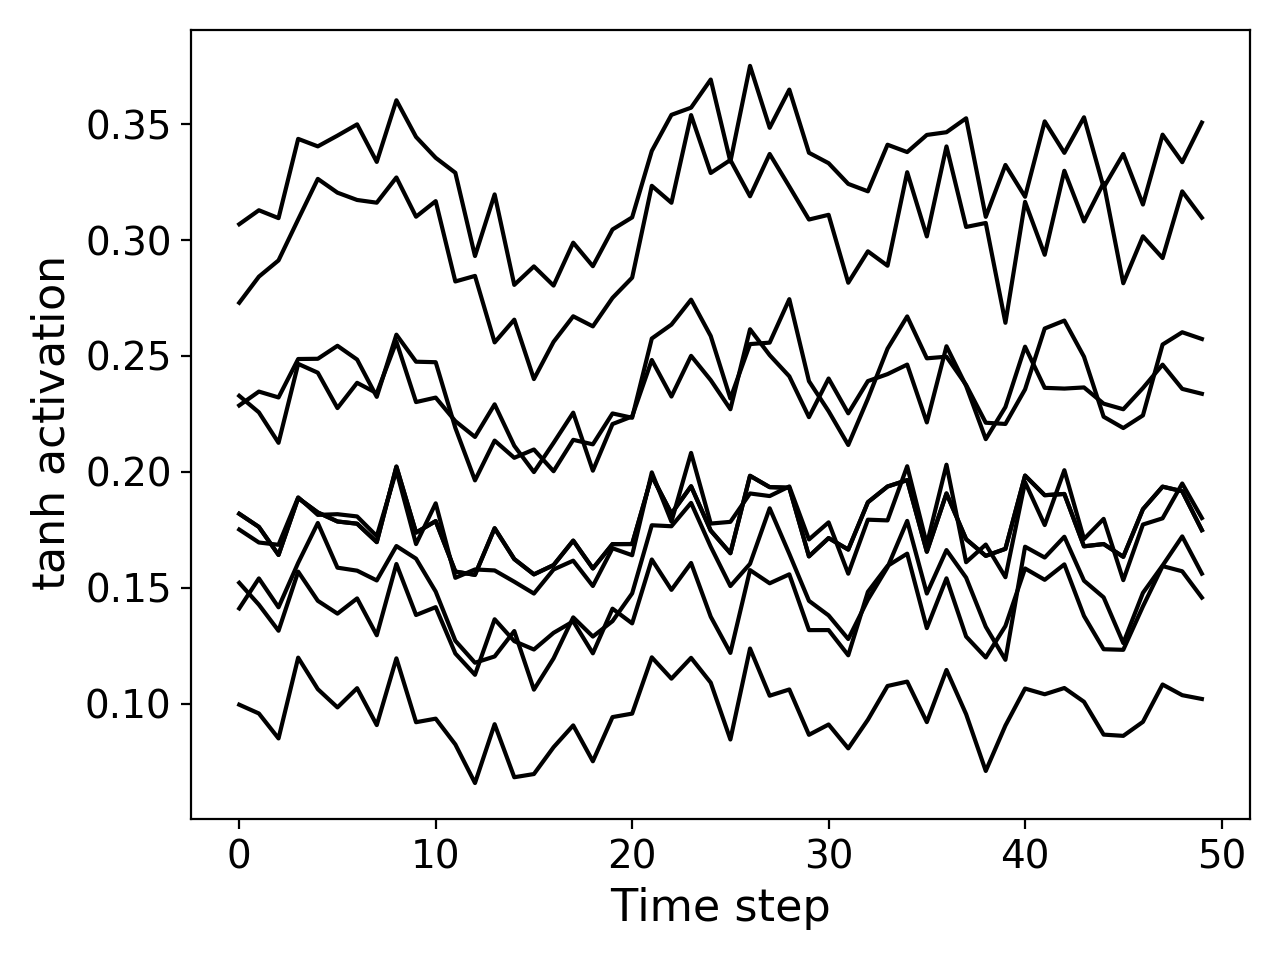
\includegraphics[width=1.0\linewidth]{figures/sq-activations.png}
    \caption{}
    \label{fig:activations-b}
  \end{subfigure}
  \caption{
    Evolution of internal node activations for ESN (a) and square lattice with
global input (b). Reservoirs contain $N = 144$ nodes, but only a subset of 10 is
shown to avoid clutter.
  }
  \label{fig:activations}
\end{figure*}

The evolution of internal node activations proves to be of interest. Figure
\ref{fig:activations} depicts an example run, comparing the standard ESN to
square grids with a fixed, global input scheme. It is clearly visible that nodes
in Figure \ref{fig:activations-b} receive the same input, while uniform
distribution of the ESN in \ref{fig:activations-a} seems more sporadic due to
its uniform input distribution in the interval [-0.5, 0.5].

Note also that the activations of nodes in a square lattice reservoir are
strictly positive, as the NARMA input sequence is strictly positive. This may
warrant a change of activation to other sigmoid functions, as half of $tanh$
remains unused, but has not been investigated further.

In summary, our experimental results demonstrate the potential of designing
reservoirs in a non-stochastic manner. By introducing directed edges to
spatially constrained lattice reservoirs, we have stumbled upon reservoirs that
perform exceptionally well on the NARMA-10 benchmark. These results suggest
that, in a physical RC context, physical substrates will show degraded
performance unless there is a directed flow of information. Additionally, we
propose directed lattice reservoirs as a means to explore this impact of
information flow deeper.

\section{Nonlinear Dynamics in Square Grids}

\subsection{Synopsis}

In this section we look at the potential diversity of nonlinear operations in
square lattice reservoirs. Although the NARMA-10 presents a task of nonlinear
operation, we herein conduct experiments to determine the kernel quality and
generalization capabilities of the square lattice reservoirs, and run benchmarks
with the Mackey-Glass benchmark to generate a mildly chaotic attractor ($\tau =
17$).

\subsection{Results and Discussion}

% (TODO): t!
\begin{figure*}[t]
  \centering
  \begin{subfigure}{.49\textwidth}
    \centering
    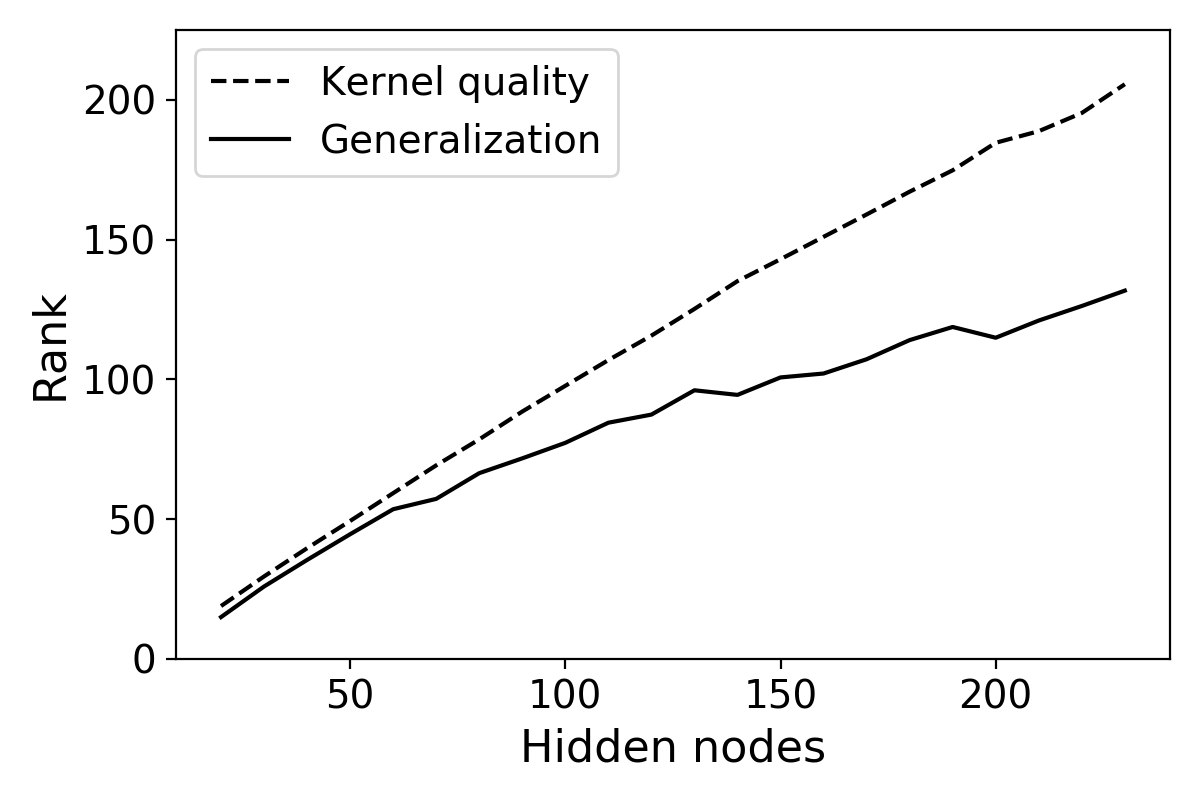
\includegraphics[width=1.0\linewidth]{figures/esn-rank.png}
    \caption{}
    \label{fig:rank-a}
  \end{subfigure}
  \begin{subfigure}{.49\textwidth}
    \centering
    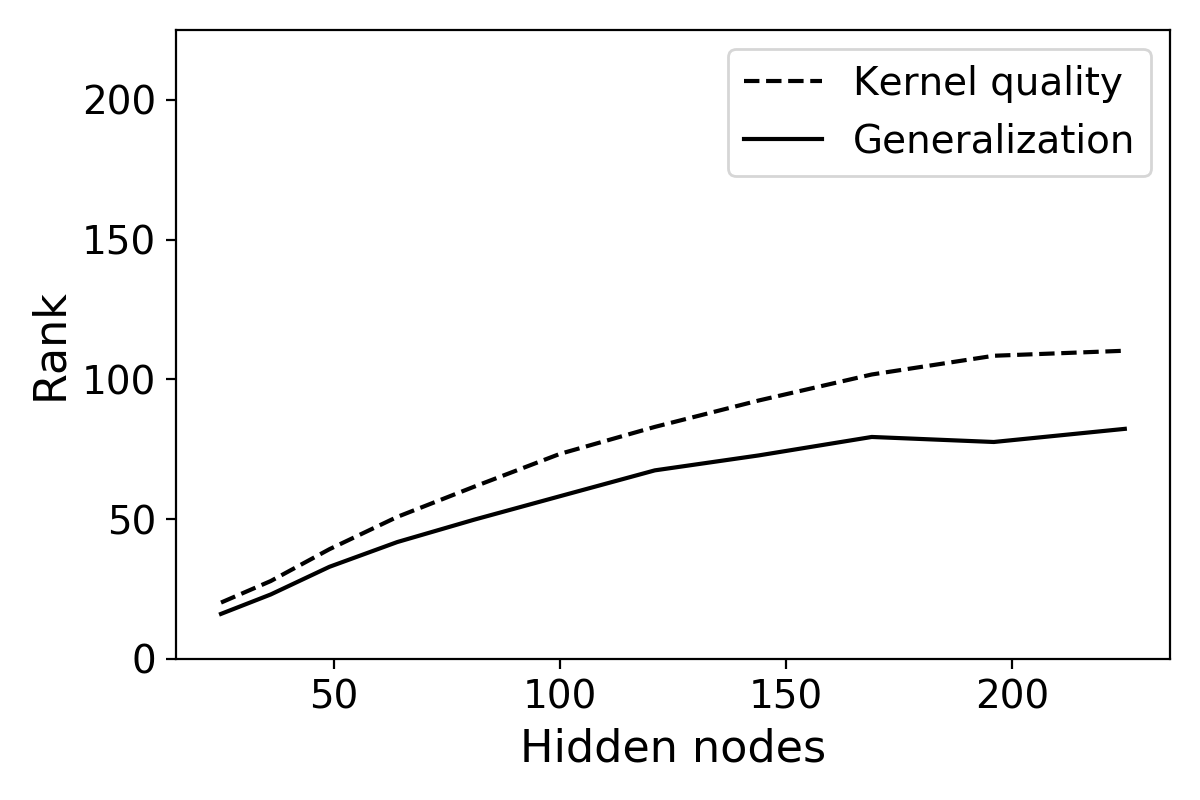
\includegraphics[width=1.0\linewidth]{figures/sq-rank.png}
    \caption{}
    \label{fig:rank-b}
  \end{subfigure}
  \caption{
    Kernel quality and generalization capability as a function of reservoir size
for ESN (a) and square lattice reservoirs (b).
  }
  \label{fig:rank}
\end{figure*}

Consider Figure \ref{fig:rank}, comparing the kernel quality of the default ESN
to square lattice reservoirs. The parameters of the reservoirs remain the same
as in Section \ref{sec:lat-dir-edge}, except a scaling of the ESN spectral
radius to 0.7, as to avoid complete saturation of the respective ranks. We
discover that square lattice reservoirs attain lower kernel
qualities. Additionally the difference between kernel quality and generalization
is also higher for ESN. This difference is often used as a metric of reservoir
quality, as a high kernel quality and low generalization rank is desirable.

If we examine kernel quality (KQ) and generalization rank (G) as a behavior
space $KQ:G$, sweeping parameter spaces will reveal the flexibility of reservoir
types. For all reservoirs, $KQ < N$ and $G < N$, given reservoir size $N$. It is
known that the standard, fully-connected ESN may be tuned to have almost any
$KQ:G$, while lattice reservoirs cover a smaller area of the $KQ:G$ behavior
space, as they are unable to achieve a high $KQ$
\cite{mcquillan_role_2019}. This conclusion is reproduced in Figure
\ref{fig:rank}.

In Section \ref{ssec:topology-and-spatial-networks}, we noted a discrepancy
between performance predicted by kernel quality and benchmarks used by Rodan and
Tiňo in their work on ring topologies. Ring topologies cover a smaller area of
the $KQ:G$ behavior space than fully-connected ESNs. Nonetheless, cyclic
reservoirs with regular jumps (CRJ) consistently outperform ESNs across multiple
benchmarks \cite{rodan_simple_2012}. We see a similar outcome in our experiments
with square lattices, where reservoirs perform comparably on the benchmark, but
exhibit a lower kernel quality. This strengthens a conclusion that
deterministically constructed reservoirs can perform well, given appropriate
tasks.

% (TODO): t!
\begin{figure}[t]
  \centering
  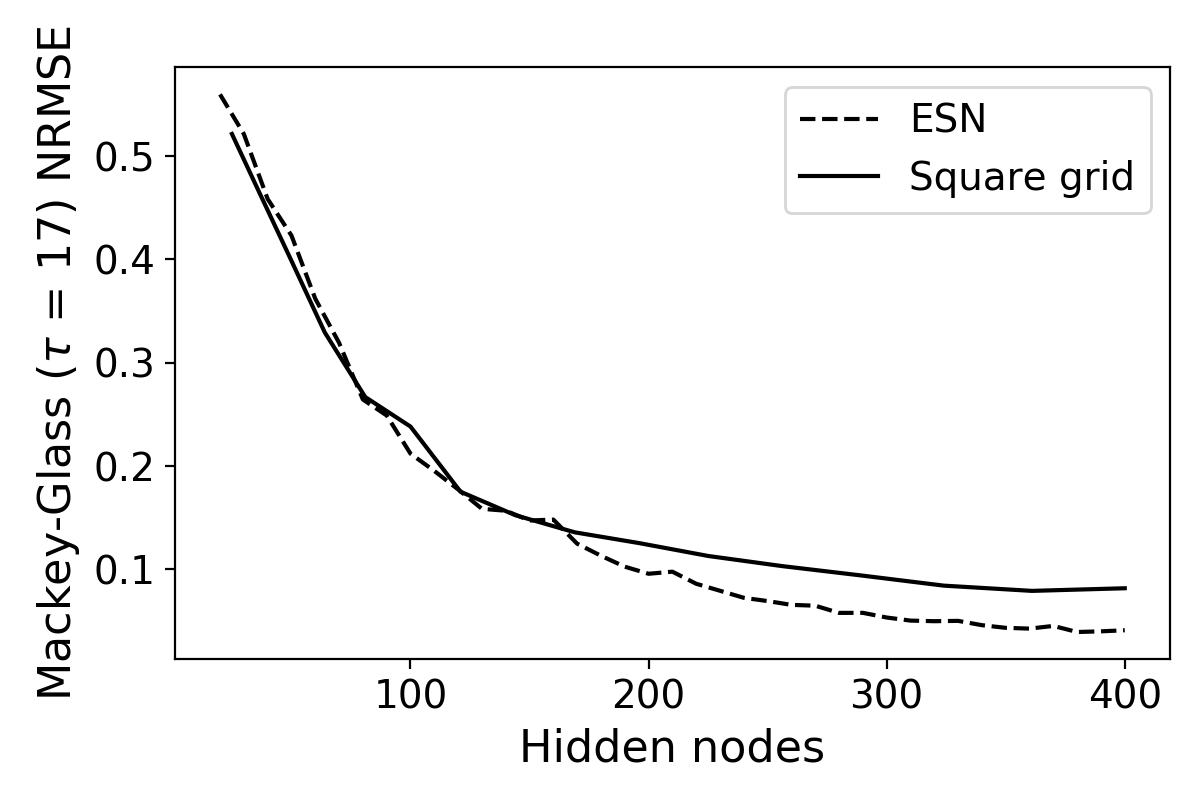
\includegraphics[width=3.5in]{figures/mg17.png}
  \caption{
    NRMSE as a function of reservoir size. Note that this benchmark is the
Mackey-Glass chaotic attractor with $\tau = 17$.
  }
  \label{fig:mg17}
\end{figure}

Figure \ref{fig:mg17} shows NRMSE achieved for square lattice reservoirs on the
Mackey-Glass delay differential equation with mild chaos, $\tau = 17$. Again,
see a comparable performance, although in this case the ESN model scales
slightly better. We would like to stress that previous work commonly compares
reservoirs up to a size of $N = 200$, in which case Figure
\ref{fig:rt-performance-big} and Figure \ref{fig:mg17} show ESN and square
lattice reservoirs to almost perform equally. Thus, from these benchmarks we may
gather that there is potential in lattice reservoirs as simulation models, most
pressingly as a tool for theoretical analysis rather than an ESN competitor.

\section{Shrinking and Growing Square Grids}
\label{sec:shrink-grow}

\subsection{Synopsis}

In Section \ref{sec:lat-dir-edge} we asserted that the directedness of square
lattice reservoirs will allow us to peer into the ``black box'' character of
reservoirs. Traditional reservoir generation is driven by ad-hoc methodology,
resulting in reservoirs which internals are difficult to interpret. Hence,
constructing simpler, more deterministic reservoirs will allow us a clearer view
of where and how input will flow in the network. Lattice reservoirs follow a
straightforward connectivity scheme and are embedded in space, making analysis
easier.

In this section we attempt to gain a deeper understanding into what makes a
square lattice reservoir perform well on the NARMA-10 benchmark. First we remove
nodes from the lattice in an incremental manner, where each iteration removes
the node that results in the lowest increase in error. Then we take the opposite
route, adding nodes along the frontier of the lattice, always adding the node
and directing the edges in the manner causing the largest decrease in
error. Both shrinking and growing square lattice reservoirs thus follow a
simplistic, exhaustive approach.

\subsection{Results and Discussion}

\subsubsection{Shrinking Reservoirs}

\begin{figure}
  \centering
  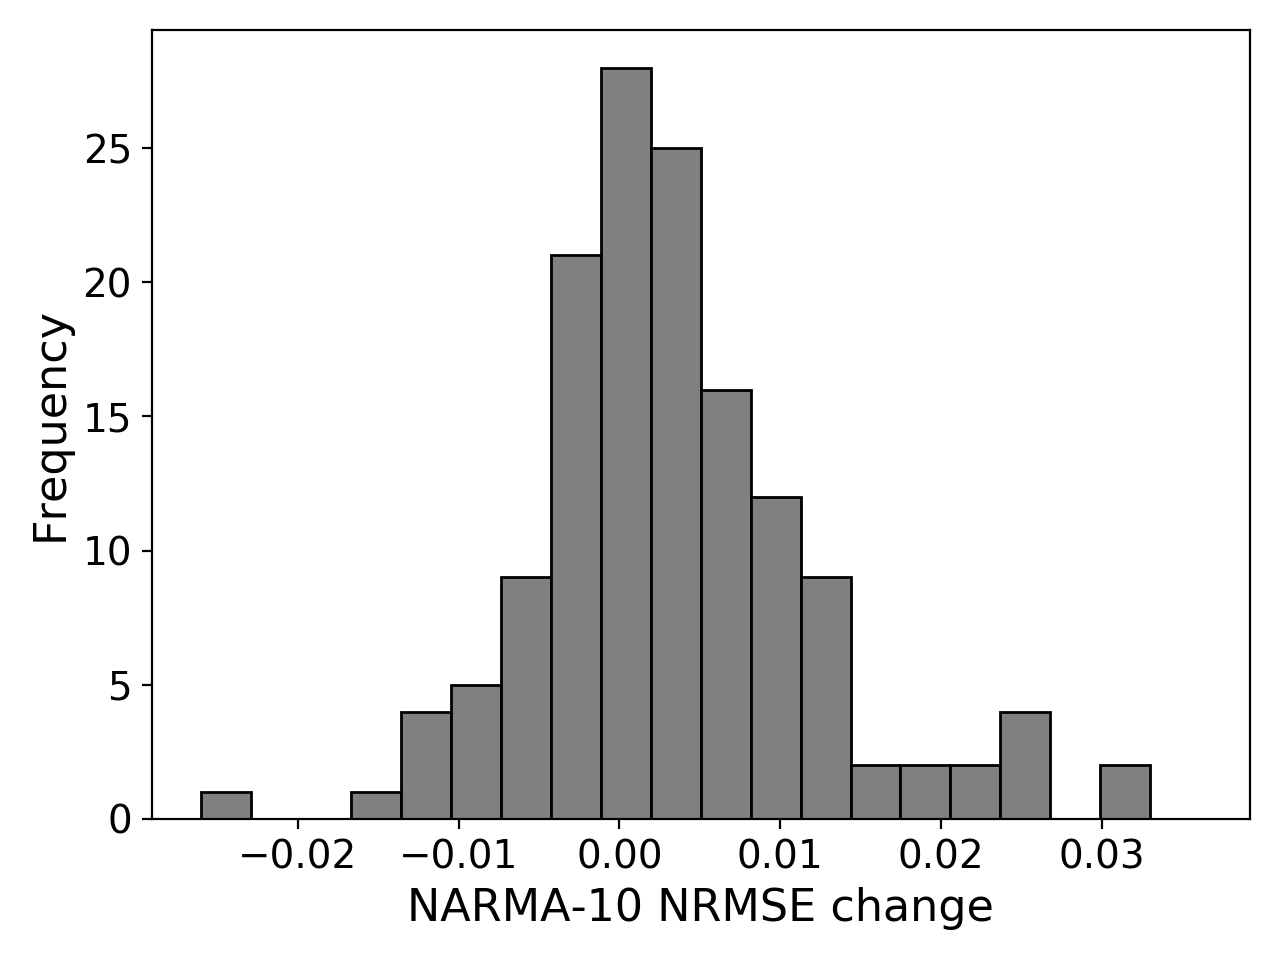
\includegraphics[width=3.5in]{figures/removal-hist.png}
  \caption{
    Impact of node removal from a $12 \times 12$ square lattice reservoir. The
original NRMSE of the reservoir is 0.28.
  }
  \label{fig:rt-removal-hist}
\end{figure}

We begin the experiment by creating a single $12 \times 12$ square lattice
reservoir and evaluating the impact of removing singular nodes in individual
copies. Figure \ref{fig:rt-removal-hist} shows the distribution of the impact
the removal of a node has on a reservoir with an original benchmark NRMSE of
0.28. Few node removals make a difference, and the few that do only change the
NRMSE marginally. This speaks to an inherent robustness in the reservoir, as
dead nodes do not degenerate performance entirely. Interestingly, a minority of
nodes provide a decrease in error upon removal, indicating a noisiness that
causes a hinderance.

\begin{figure}
  \centering
  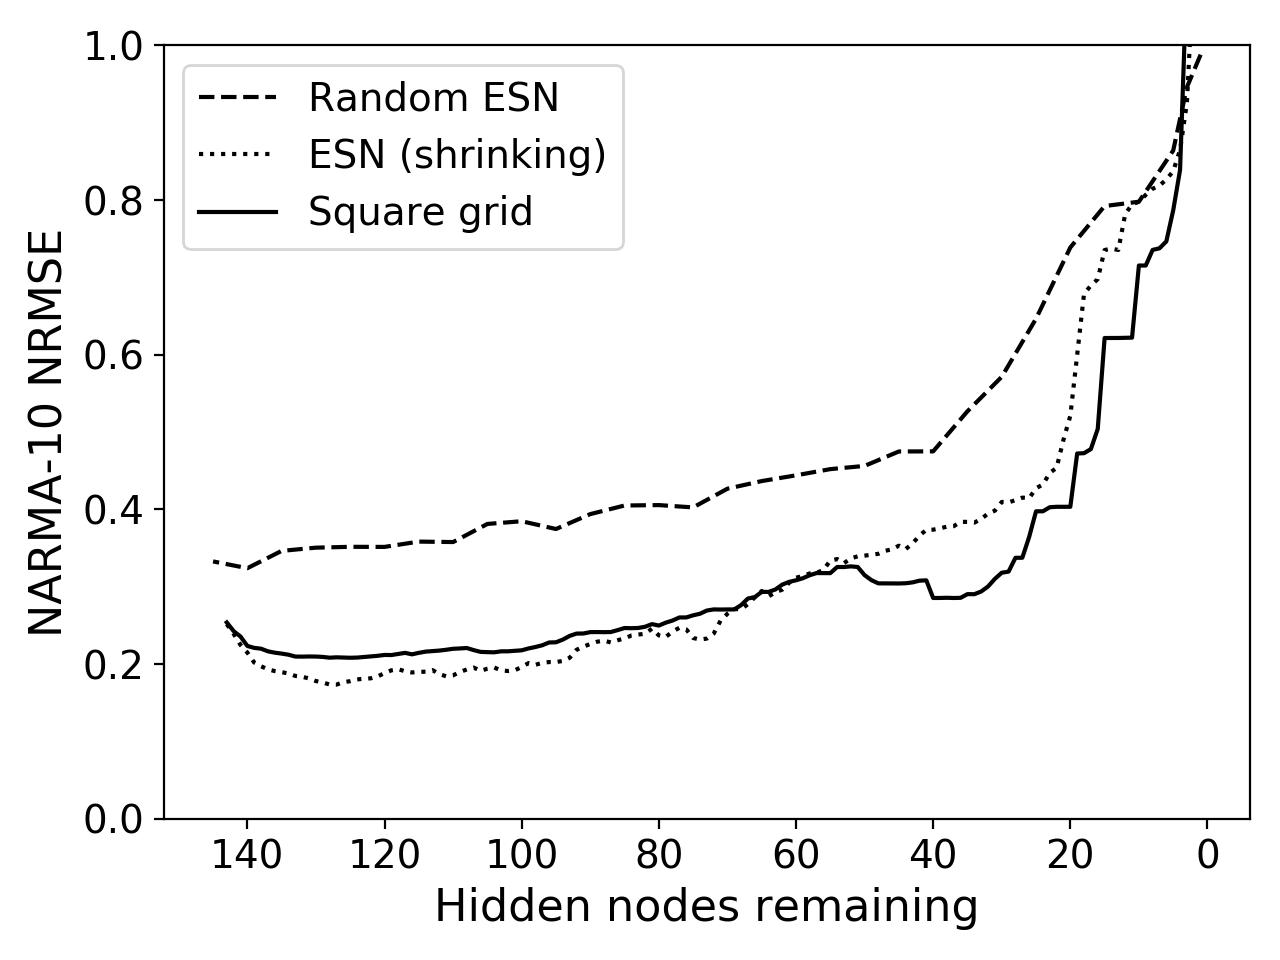
\includegraphics[width=3.5in]{figures/shrink-performance.png}
  \caption{
    NRMSE as a function of nodes removed from the original reservoir. Both
traditional ESN and square lattice reservoirs are investigated, and compared to
randomly a randomly generated ESN of the same size.
  }
  \label{fig:sq-shrink-performance}
\end{figure}

When node removals have been exhausted, the node causing the smallest increase
in benchmark error is removed. This is then repeated until there is a single
node left in the reservoir. Figure \ref{fig:sq-shrink-performance} details the
development of reservoir error for each iteration. We conduct the same
experiment with default ESNs, comparing both models to randomly generated ESNs
of the same size.

Results show that both square lattice reservoirs and ESN reservoirs benefit from
removal of a few noisy nodes. Furthermore, almost half the reservoirs may be
removed in this manner before performance degrades to values below that of the
initial state. Clearly, numerous of the hidden nodes in the reservoirs that were
generated originally serve little purpose. Pruning ESNs has been attempted
before. For example, by pruning output connections as regularization methods
\cite{dutoit_pruning_2009}, or by using the concept of attack tolerance to
remove nodes which output weights $\mathbf{W}^{out}$ correspond to large or
small values \cite{haluszczynski_reservoir_2020}. Results that indicate
optimization potential in network pruning are interesting in a physical RC
context, as the resources required to realize reservoirs naturally increases
with size.

% (TODO): t!
\begin{figure*}[t]
  \centering
  \begin{subfigure}{.40\textwidth}
    \centering
    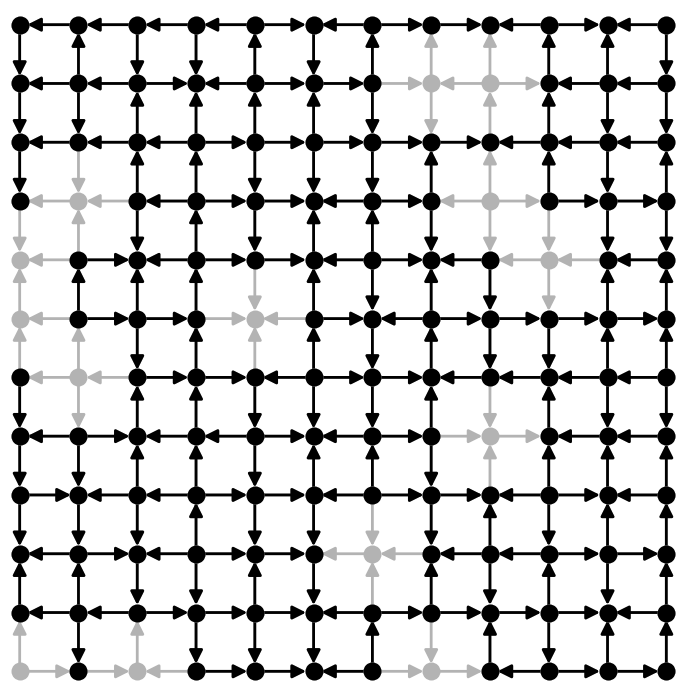
\includegraphics[width=1.0\linewidth]{figures/sq-grid-130.png}
    \caption{$N = 130$, NRMSE = 0.21.}
    \label{fig:sq-grid-130}
  \end{subfigure}
  \begin{subfigure}{.40\textwidth}
    \centering
    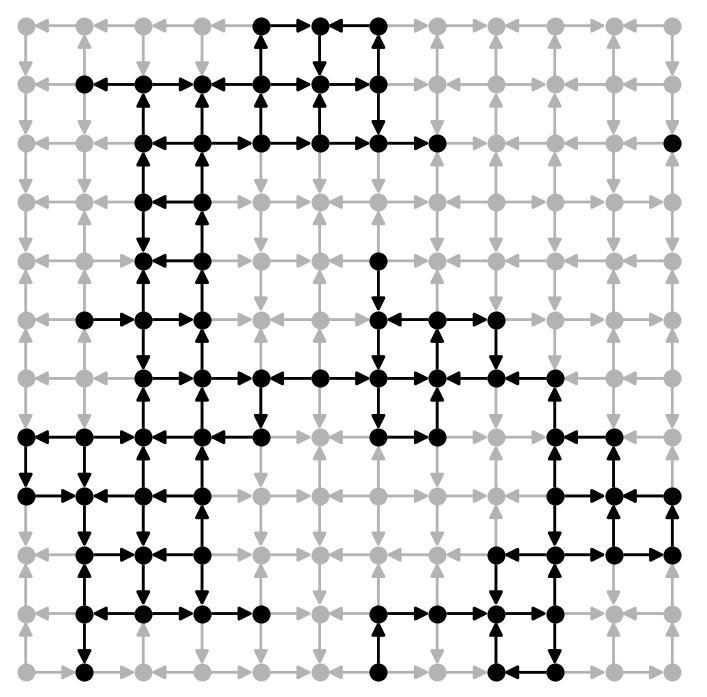
\includegraphics[width=1.0\linewidth]{figures/sq-grid-70.png}
    \caption{$N = 70$, NRMSE = 0.27.}
    \label{fig:sq-grid-70}
  \end{subfigure}
  \vskip\baselineskip

  \begin{subfigure}{.40\textwidth}
    \centering
    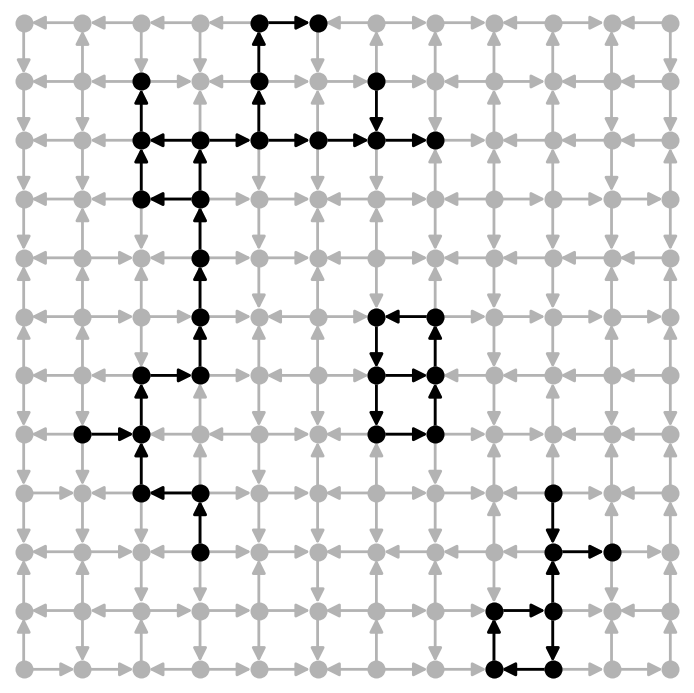
\includegraphics[width=1.0\linewidth]{figures/sq-grid-35.png}
    \caption{$N = 35$, NRMSE = 0.29.}
    \label{fig:sq-grid-35}
  \end{subfigure}
  \begin{subfigure}{.40\textwidth}
    \centering
    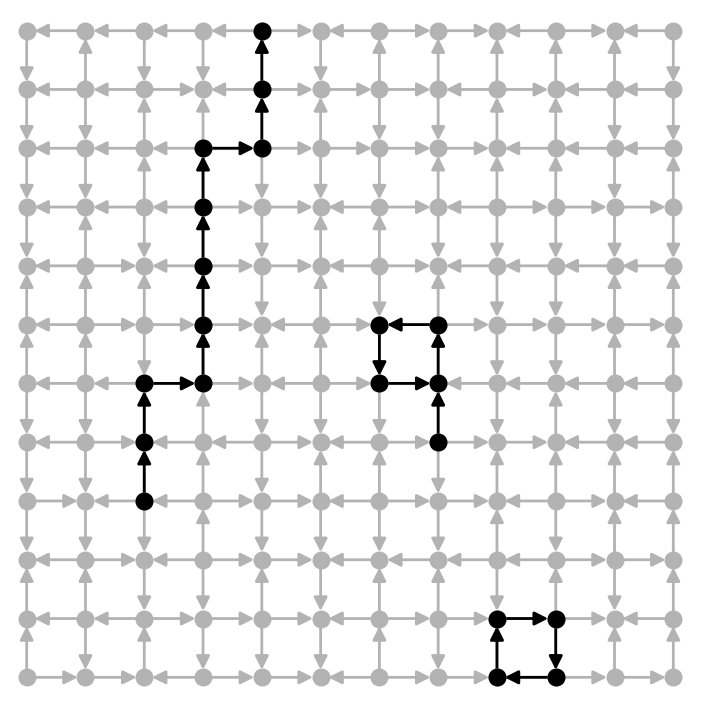
\includegraphics[width=1.0\linewidth]{figures/sq-grid-20.png}
    \caption{$N = 20$, NRMSE = 0.40.}
    \label{fig:sq-grid-20}
  \end{subfigure}
  \caption{
    Evaluation during incremental removal of nodes from a $12 \times 12$ square
lattice reservoir.
  }
  \label{fig:sq-grid}
\end{figure*}

Pruning reservoir size is relevant not only to reduce costs, it is also valuable
for theoretical analysis. Figure \ref{fig:sq-grid} depicts the state of the
reservoir at four different points during shrinking. Performance degrades to
that of a delay line when there is around $N = 20$ nodes left in the reservoir,
shown Figure \ref{fig:sq-grid-20}. This is also exactly what is remaining: a
delay line of length 11, and two cycles of length 4. Moreover, an NRMSE of 0.29
achieved with just $N = 35$ nodes in Figure \ref{fig:sq-grid-35}. We see a
``core'' providing the required short-term memory, with nodes along this stem
for processing purposes. This core is also present in the original 144-node
network, but is now easier to spot.

We have illustrated the value of square lattice reservoirs as an analytical
tool. This rather simple experiment has deduced that heavy lifting to solve the
NARMA-10 benchmark is done by a core stem of memory augmented by surrounding
nodes. A comparable analysis is harder to make for the corresponding shrunk ESN
reservoir from Figure \ref{fig:sq-shrink-performance}, as even just embedding
the network in a metric space requires complicated spring models such as
force-directed graph drawing.

In summary, in this section we have deviated slightly from the original goal of
the thesis relating spatial constraints to physical substrates to investigate
the spatial structures that emerge in lattice reservoirs that solve the NARMA-10
benchmark. We suggest the analysis herein to be only the tip of the iceberg, as
heuristics such as average node degree, investigation of the cyclic structures,
and adding skip edges to square lattices to improve our understanding of the ESN
black box.

\subsubsection{Growing Reservoirs}

Growing reservoirs in the same manner as shrinking them is an enticing
approach. There is a finite amount of positions where new nodes may be inserted
into the network, and for each such position there is only a handful of ways to
direct the incident edges. By exhausting all possibilities, we may attach the
node that causes the largest decrease in benchmark error.

\begin{figure} \centering
  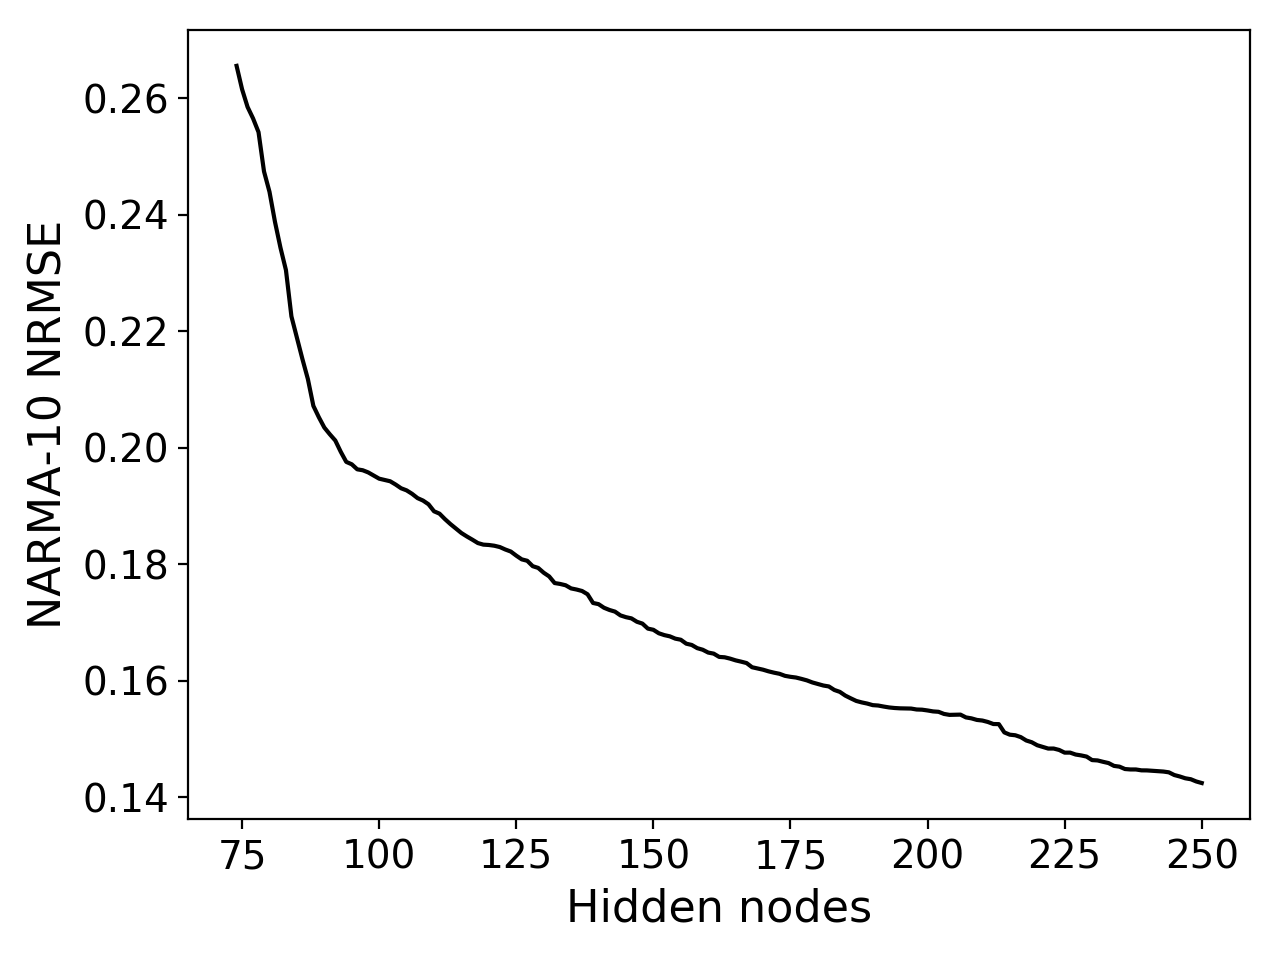
\includegraphics[width=3.5in]{figures/grow-performance.png}
  \caption{
    NRMSE as a function of hidden nodes when growing a square lattice
reservoir. The process is begun from a reservoir of size $N = 74$, depicted in
Figure \protect\ref{fig:sq-grid-grow-74}.
  }
  \label{fig:sq-grow-performance}
\end{figure}

Figure \ref{fig:sq-grow-performance} shows the NRMSE development of a reservoir
grown with this method. We begin with a node of $N = 74$ hidden nodes, found to
be the best performing reservoir when shrinking a $12 \times 12$ square lattice
reservoir in the previous section. We see a steady decrease in benchmark error
for each node addition. Achieving a great benchmark score is of course
desirable, as the results clearly show that building reservoirs specialized for
specific tasks will outperform randomly generated ones.

% (TODO): t!
\begin{figure*}[t] \centering
  \begin{subfigure}{1.0\textwidth} \centering
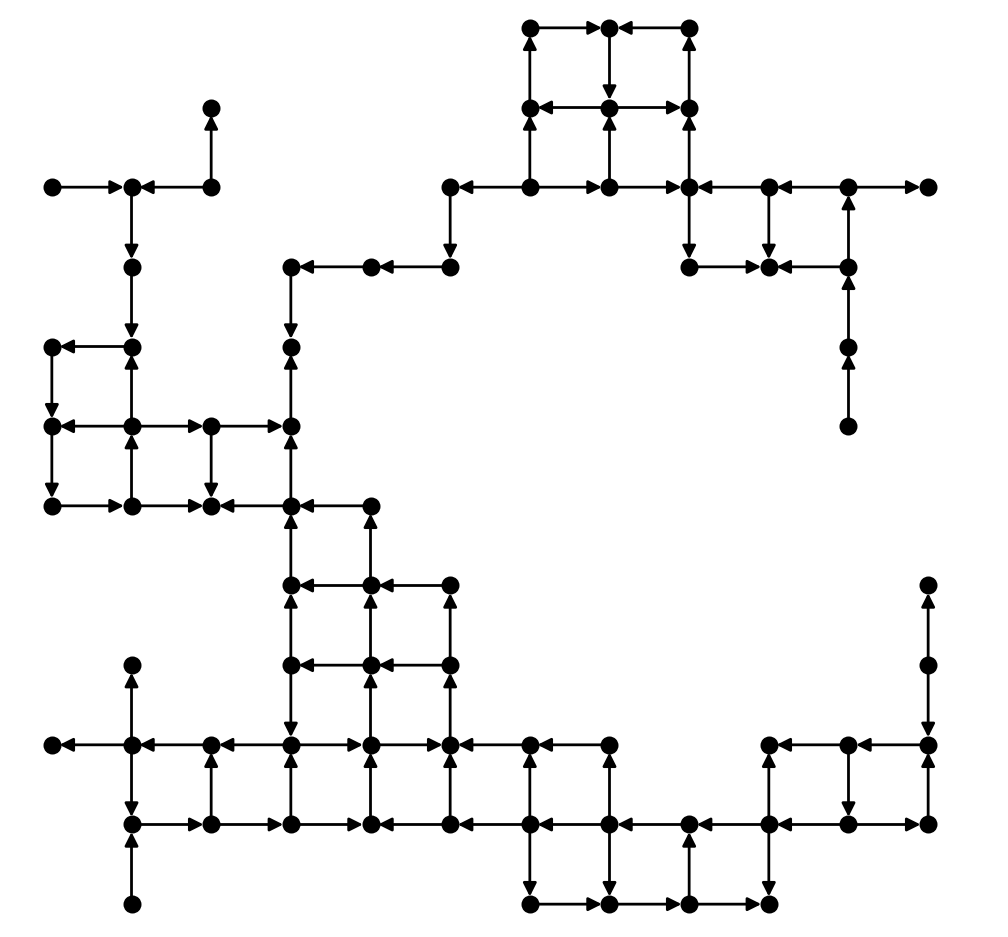
\includegraphics[width=0.5\linewidth]{figures/sq-grid-grow-74.png}
    \caption{$N = 74$, NRMSE = 0.26.}
    \label{fig:sq-grid-grow-74}
  \end{subfigure}
  \begin{subfigure}{.49\textwidth} \centering
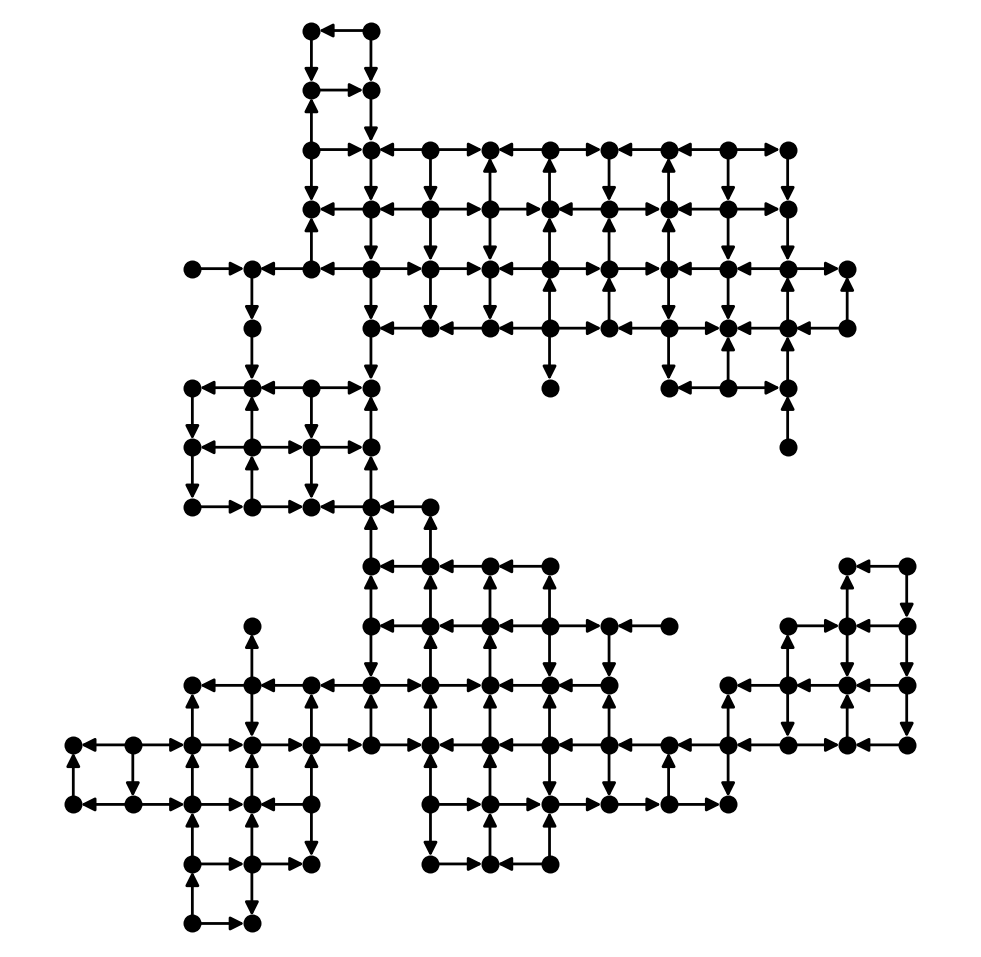
\includegraphics[width=1.0\linewidth]{figures/sq-grid-grow-124.png}
    \caption{$N = 124$, NRMSE = 0.18.}
    \label{fig:sq-grid-grow-124}
  \end{subfigure}
  \begin{subfigure}{.49\textwidth} \centering
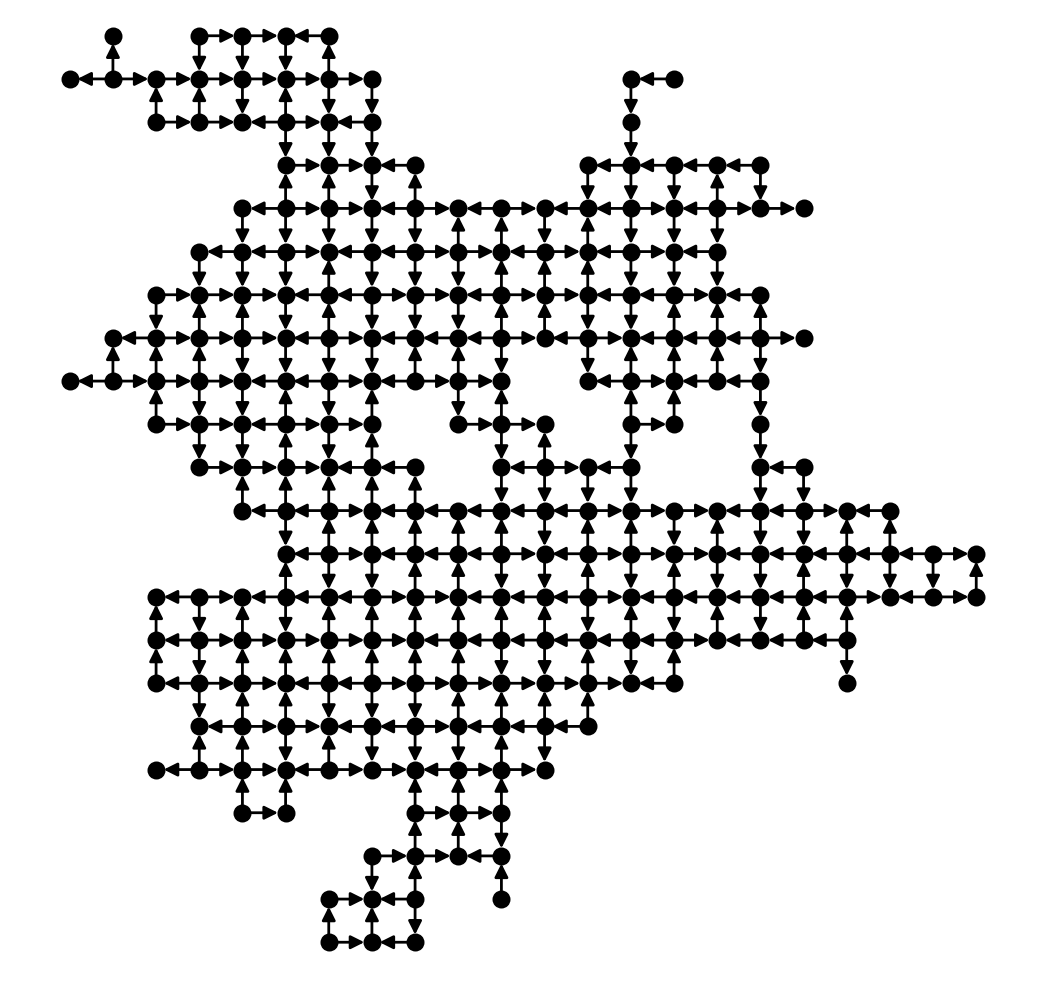
\includegraphics[width=1.0\linewidth]{figures/sq-grid-grow-250.png}
    \caption{$N = 250$, NRMSE = 0.15.}
    \label{fig:sq-grid-grow-250}
  \end{subfigure}
  \caption{
    Evaluation during incremental addition of nodes to a square lattice
reservoir. The process starts from the reservoir in (a).
  }
  \label{fig:sq-grid-grow}
\end{figure*}

However, as previously mentioned, our intention with square lattice reservoirs
is not to provide yet another ESN competitor, but to gain insights into their
inner workings. Figure \ref{fig:sq-grid-grow} depicts the reservoir at three
different points during its growth. Curiously, holes appear in the lattice in
Figure \ref{fig:sq-grid-grow-250}, demonstrating that there are parts of the
lattice where adding nodes, irrelevant of the directions of its incident edges,
will cause little performance gain.

Figure \ref{fig:sq-grid-grow-250} also illustrates the apparent difficulty of
analyzing networks without good heuristics. Consider for example the difference
between Figure \ref{fig:sq-grid-grow-250}, and the much smaller Figure
\ref{fig:sq-grid-35}. The latter provides a much clearer picture of what it is
\textit{doing} during the NARMA-10 benchmark. We thus refer to the approaches
suggested in the summary of the previous section -- there seems to be tremendous
potential in researching the creation of structured, deterministic reservoirs.

\section{Restoring Bidirectional Edges}

\subsection{Synopsis}

Among the discoveries of our previous experiments, the importance of directed
edges to create a flow of information is of major relevancy to physical RC
settings. In this section we analyze the effect of restoring bidirectional edges
by following the greedy approach in Section \ref{sec:shrink-grow}. A base $12
\times 12$ square lattice reservoir is generated, and its 264 edges are
incrementally made bidirectional by choosing the edge causing the least increase
in error for each iteration.

\subsection{Results and Discussion}

\begin{figure}
  \centering
  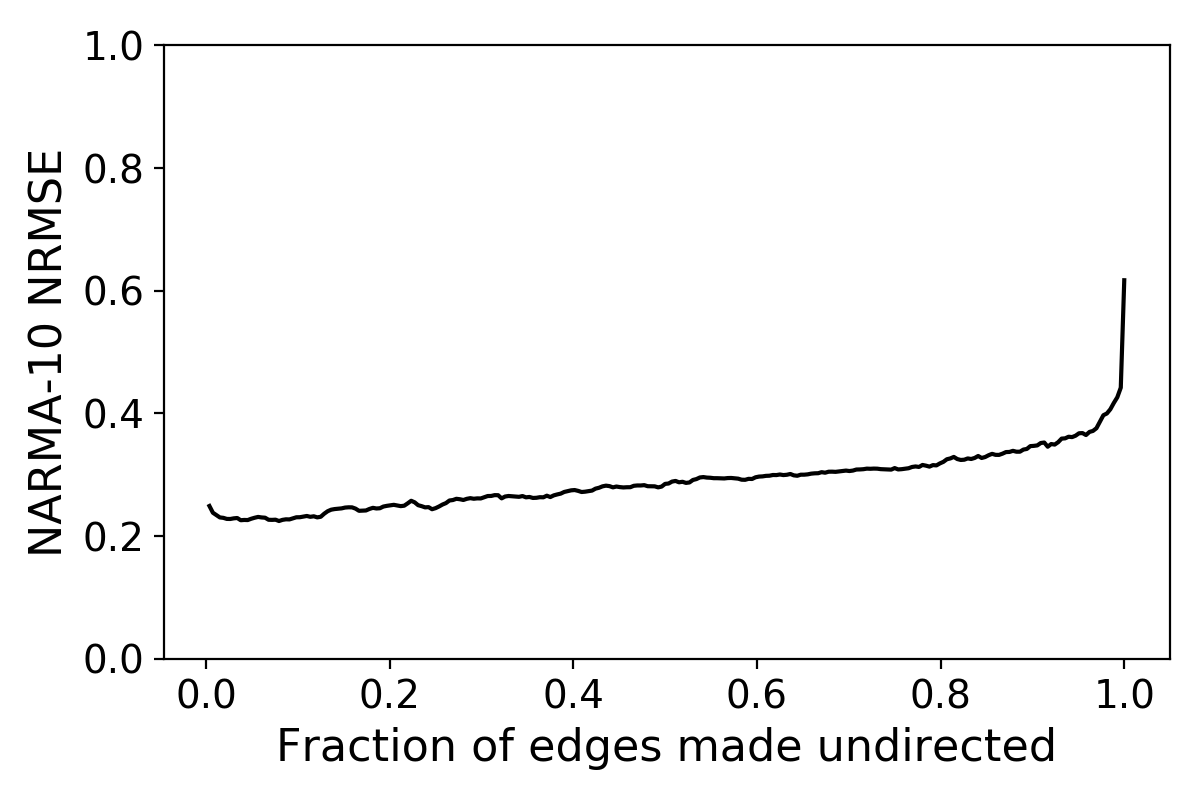
\includegraphics[width=3.5in]{figures/undir-performance.png}
  \caption{
    NRMSE as a function of the fraction of edges of a square lattice reservoir
that are changed to be undirected. A $12 \times 12$ lattice is used, starting
from 264 directed edges.
  }
  \label{fig:undirection-performance}
\end{figure}

Results are shown in Figure \ref{fig:undirection-performance}. First, there is a
small dip in error for the initial 20 or so edges. When an edge goes from
directed to undirected, its entry in $\mathbf{W}^{out}$ is in practice mirrored
along the diagonal axis, essentially \textit{adding} an incident edge in the
opposite direction. When greedily choosing which edges to change, it is
unsurprising that there are instances where an additional edge is beneficial.

As an increasing fraction of edges made undirected, the reservoir benchmark
error rises steadily. Performance degrades drastically after about 90\% of edges
have been changed. Again we see that a non-symmetric weight matrix enables
richer dynamics, here as a direct consequence of the restored symmetry.

\section{Conclusions}

\textcolor{red}{
  Remember that we are not necessarily concerned with finding really good square
grids, but rather that they work at all, since we are concerned with spatial
constraints.
}

\textcolor{red}{
  We find square grids to slightly outperform ESNs on NARMA, and about as good
on MG17.
}

\textcolor{red}{
  We find directedness to be important, and \textit{sufficient}. We find a type
of ESN that is fairly deterministic like CRJ, but has some freedom in
structure. This is useful for exploring ESNs.
}

\textcolor{red}{
  We underline a discrepancy between KQ and actual performance that is already
seen with CRJ. This is quite interesting.
}

\textcolor{red}{
  By analyzing removal of nodes, we find that there seems to be a ``core'' stem
for solving the NARMA task. And ``augmenting'' nodes around. This might be
telling about what happens in ESNs also, but due to randomness.
}

\textcolor{red}{
  We find that removing nodes and evaluating can be good to remove noisy nodes.
}


%%% Local Variables:
%%% mode: latex
%%% TeX-master: "../thesis"
%%% End:

\chapter{Experiments: Towards Artificial Spin Ice}

Experiments that resemble ASI.

%%% Local Variables:
%%% mode: latex
%%% TeX-master: "../thesis"
%%% End:

\chapter{Conclusion and Future Work}
\label{ch:conclusion}

\section{Conclusion}

In this thesis we have explored physical reservoir computing with spatial
constraints. Our goal was to provide a better theoretical foundation for how
reservoir computing methodology translates to physical substrates. We conducted
software simulations using echo state network methodology to investigate the
feasibility of reservoirs with two different spatial restrictions: random
geometric graphs and lattices. Furthermore, we have developed lattice reservoirs
that can be used for theoretical analysis of ESN internals, accompanied with
example analyses of deterministic reservoir construction.

\textbf{RQ1:} How does the reservoir computing paradigm translate to the
spatially constrained topology setting of a physical medium?

The difference from abstraction models such as ESNs to physical reservoirs is
primarily concerned with the \textit{limitations} posed when interacting with an
actual physical substrate. In this work we have investigated spatial
limitations, and in Section \ref{sec:rwd} we emphasized that the weight
distribution resulting from a spatially constrained reservoir is different from
unrestricted architectures. The translation of the RC paradigm to a spatial,
physical setting is thus primarily limited by the (possibly fixed) geometries of
the underlying substrate how its internal units are connected. Other limitations
than spatial constraints, such as noise and system observability, were explored
in preliminary work \cite{aven_exploring_2019}.

More specifically, we have shown that ESNs with imposed spatial limitations by
default see a decrease in performance compared to their abstract
counterparts. However, both RGG and lattice reservoirs achieved improved
performance once the symmetry in the resulting internal reservoir matrix was
broken by directed and signed edges.

\textbf{RQ2:} How do highly regular, physical structures compare in information
processing capability to that of established models such as echo state networks?

Highly regular lattice structures with \textit{bidirectional} edges perform
worse than ESNs. However, our investigations also demonstrated that introducing
directedness to lattice reservoirs restores the ESN performance, indicating that
structures that allow a definitive flow of information may be sufficient. We
also showed that a fixed, global input betters performance compared to a
standard uniform distribution, making lattice reservoirs scale better than
traditional ESNs on the NARMA-10 benchmark. We thus observe that regular
structures may perform just as well as established models, as both previous work
on ring topology as well as the work in this thesis suggests that
deterministically constructing regular reservoirs has revealed great potential.

\textbf{RQ3:} Can we find simple, deterministic reservoir generation
methodology, relying less on random weighting schemes?

It is previously established that ring topology models may be constructed
deterministically to serve as quality reservoirs \cite{rodan_minimum_2011}. In
this thesis we introduced lattice reservoir models, which are constructed by
deterministically placing nodes on a two-dimensional grid. Both ring and lattice
reservoirs, however, require some stochastic element to work well. In the case
of rings the sign of the input seen by each node is determined by an unbiased
coin, while in the case of lattices it is the direction of the edge between each
node that is decided by a coin flip. We therefore argue that there is untapped
potential in creating reservoirs of deterministic, regular natures.

Finally, by removing and adding nodes to lattice reservoirs, we illustrated
methodology for theoretical analysis of the inner workings of such
networks. Firstly, we found that a removal of a few nodes can be a convenient
measure to reduce network size and improve prediction performance. More
importantly, we also argue that understanding the behavior of networks when
solving specific benchmarks is a stepping stone to looking into the general
black box behavior of ESNs, and that the regular structure of lattice reservoirs
is easier to observe directly than the more stochastic structure of ESNs. Hence,
the intention of lattice reservoirs is not to provide yet another ESN
competitor, but to open up for further analysis in future work.

\section{Future Work}

As there is always an abundance of future work to conduct, we here limit
suggestions to two main categories of experiments we deem the most interesting
to explore: physical realization of reservoirs to determine if directed exchange
and flow of information is sufficient to create quality reservoirs, and deeper
theoretical analysis using lattice models to find interesting heuristics in good
reservoirs.

First, as ASI has proven to be a promising substrate for reservoir computing, it
is a good candidate for study of real physical limitations
\cite{jensen_reservoir_2020}. In this thesis it is suggested that directedness
is a key component in good reservoirs, and how this translates to an actual
physical medium would be interesting to explore. For example, imposing shift
register structures onto ASI to allow for directed flows may hold a potential
for creating quality reservoirs.

Second, further theoretical analysis using lattice models should result in a
deeper understanding of why the traditional, stochastic ESN model works so
well. By modifying lattice models to find good heuristics such as average node
degree, investigate cyclic structures, add skip edges, and so on, we may
discover what it is that makes ESN reservoirs ``tick''. Specifically, lattice
reservoirs are inherently embedded in space, making them easier to visualize and
understand. This is valuable when attempting to understand how specific tasks
are solved by an ESN.

%%% Local Variables:
%%% mode: latex
%%% TeX-master: "../thesis"
%%% End:

\bibliographystyle{ieeetr}
\bibliography{ref}

\appendix
\chapter{Appendix A}



%%% Local Variables:
%%% mode: latex
%%% TeX-master: "../thesis"
%%% End:

\end{document}

%%% Local Variables:
%%% mode: latex
%%% TeX-master: t
%%% End: